\documentclass[a4paper, 11pt, titlepage]{article}
\usepackage[margin = 1in]{geometry}

\usepackage{amsmath}
\usepackage{amssymb}

\usepackage{hologo}

\usepackage{graphicx}
\graphicspath{{Figures/}}

\usepackage{datetime}
\newdate{date}{20}{01}{2018}

\usepackage{setspace}
\onehalfspacing

\usepackage[colorlinks = false, linkcolor = black]{hyperref}

\usepackage{fancybox}

\usepackage{xeCJK}
\setCJKmainfont{Songti SC}
\setmainfont{Times New Roman}

\usepackage{indentfirst}
\setlength{\parindent}{2em}

\usepackage{enumitem}
\setitemize[0]{leftmargin = 1em, itemindent = 1em}

\usepackage{listings}

\usepackage{xcolor}

\definecolor{commentsColor}{rgb}{0.497495, 0.497587, 0.497464}
\definecolor{keywordsColor}{rgb}{0.000000, 0.000000, 0.635294}
\definecolor{stringColor}{rgb}{0.558215, 0.000000, 0.135316}

\lstset{
backgroundcolor = \color{white},
basicstyle = \footnotesize,
breakatwhitespace = false,
breaklines = true,
captionpos = b,
commentstyle = \color{commentsColor}\textit,
frame = tb,
keepspaces = true,
keywordstyle = \color{keywordsColor}\bfseries,
numbers = left,
numbersep = 5pt,
numberstyle = \tiny\color{commentsColor},
rulecolor = \color{black},
showspaces = false,
showstringspaces = false,
showtabs = false,
stepnumber = 1,
stringstyle = \color{stringColor},
tabsize = 2,
title = \lstname,
columns = fixed
}

\usepackage{tcolorbox}

\author{张好 / Hao ZHANG\thanks{haozhang@me.com}}
\title{适用于 Mac OS 系统的第一份 \LaTeX 学习文档}
\date{\displaydate{date}}



\DeclareMathOperator{\argh}{argh}
\DeclareMathOperator*{\nut}{Nut}



\begin{document}

\maketitle

\tableofcontents
\newpage

\section{\LaTeX 软件的安装和使用} 

\subsection{从 \href{https://www.latex-project.org/}{\LaTeX} 的官网安装适用于 Mac OS 的 MacTeX}

\LaTeX 是基于 \textbf{\textit{LaTeX Project Public License (LPPL)}} 条款下的免费软件(\textbf{Figure 1})。\LaTeX 本身并不是一个独立的排版程序,而是基于 \textit{Donald E. Knuth} 的 \TeX 排版系统所运行的文档准备软件。 \TeX 发行版通常将运行 \TeX 系统所需的所有部件捆绑在一起,并且通常会添加这两者的配置和维护程序。如今, \LaTeX 及其上的许多软件包构成了任何 \TeX 发行版的重要组成部分。\par

\begin{figure}[hbtp]
\centering

\includegraphics[width = 16cm]{Figure_01.png}
\caption{通过 The \LaTeX Project 官网下载 \LaTeX 软件}
\end{figure}

\vspace{-2em}

\textbf{\begin{itemize}
\item[•]{\TeX 发行版的安装}
\end{itemize}}

\setlength{\leftskip}{2em}
对于一个 \TeX 和 \LaTeX 的新手或者只是想简单安装 \LaTeX 的用户而言,可以直接安装完整的 \TeX 发行版。 \TeX 用户组( \textbf{\textit{TUG}})有一个值得注意的分布清单,可以自由选择完全安装或只安装最重要的部分。\par

\vspace{-1em}

\textbf{\begin{itemize}
\item[•]{四个 \LaTeX 运行平台}
\end{itemize}}

不同平台的 \LaTeX 发行版软件,可以分别适用于 Linux、Mac OS、Windows 以及 Online 这四种操作系统或平台(\textbf{Figure 2})。包括支持 Linux 系统的 TeX Live;支持 Mac OS 系统的 MacTeX;支持 Windows 系统的 MiKTeX、proTeXt 或者 TeX Live以及支持 Online 编辑的Papeeria、Overleaf、ShareLaTeX、Datazar 和 LaTeX base。\par

\begin{figure}[hbtp]
\centering
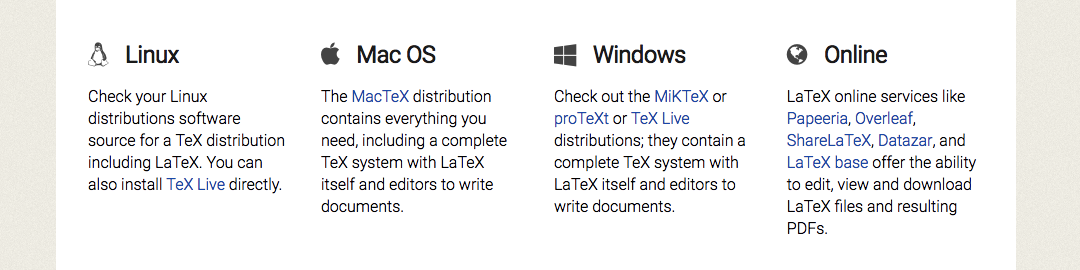
\includegraphics[width = 16cm]{Figure_02.png}
\caption{支持四种不同平台的 \LaTeX 发行版软件}
\end{figure}

\vspace{-1em}

\setlength{\leftskip}{0em}\subsection{安装适用于 Mac OS 系统的 \href{http://www.xm1math.net/texmaker/index_fr.html/}{Texmaker} 和/或 \href{https://www.texstudio.org/}{TeXstudio}}

Texmaker 是一个自由且免费的 \LaTeX 编辑器,支持 unicode,拼写检查,自动完成和代码折叠。 它集成了一个集成的 pdf 显示屏,支持 synctex 并以连续模式显示。TeXstudio 是一个用于创建 \LaTeX 文档的集成书写环境,与 Texmaker 相似,TeXstudio 也是一个自由且免费的 \LaTeX 编辑器。 对于这两个 \LaTeX 编辑器的选择,完全可以由用户的使用体验和使用习惯而定,两者各有优劣。\textbf{以下若无特殊说明,均以 Texmaker 为例。}\par

无论是使用 Texmaker 还是使用 TeXstudio,为了迎合中文的排版,通常所推荐的排版工具主要为 XeLaTeX。需要注意的是,TeX 和 pdfTeX 这两个排版工具是不直接支持 Unicode 字符的引擎,而 XeTeX 和 XeLaTeX 这两个引擎可以直接支持 Unicode 字符,因此对于中文排版的效果更为优秀。因此为了方便使用,可以将快速构建命令设置为“\textbf{XeLaTeX + 查看 PDF}”(\textbf{Figure 3})。\par

\begin{figure}[hbtp]
\centering
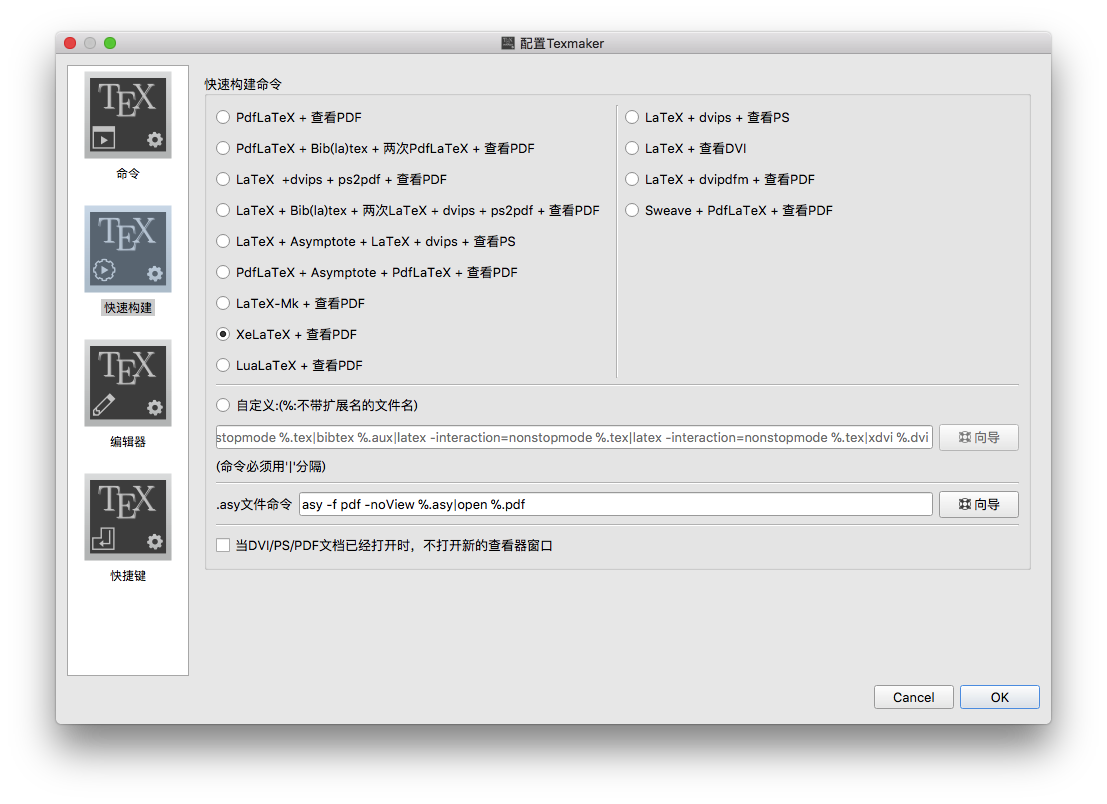
\includegraphics[width = 14cm]{Figure_03.png}
\caption{Texmaker 快速构建框中快速构建命令的设置}
\end{figure}

除外,为了方便观察 \LaTeX 编辑器的编辑效果,可以将命令中的 PDF 的查看器设置为“\textbf{内置常看器 + 嵌入}”(\textbf{Figure 4})。\par

\begin{figure}[hbtp]
\centering
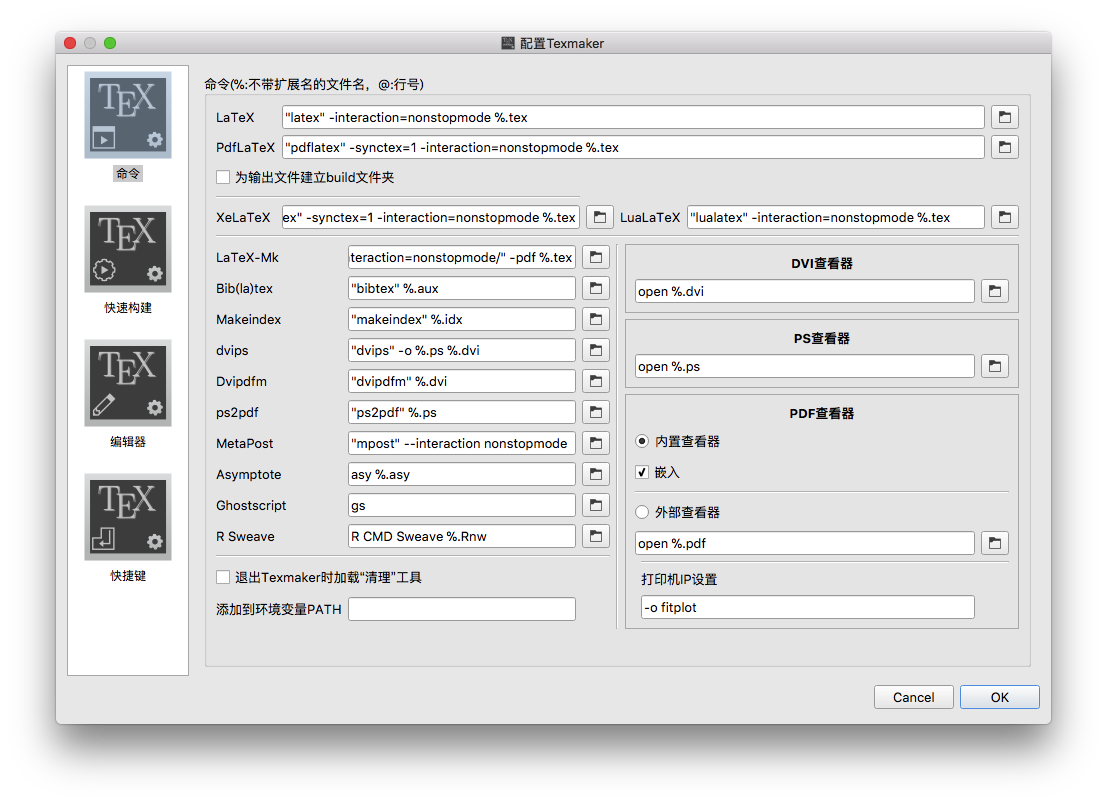
\includegraphics[width = 14cm]{Figure_04.png}
\caption{Texmaker 命令框中 PDF 内置查看器的设置}
\end{figure}

\section{了解 \LaTeX 的第一步}

\subsection{编辑第一个 \LaTeX 文档}

\begin{enumerate}
\item 打开 Texmaker,检查编辑器框中编辑器字体编码是否为 \ovalbox{UTF-8}。若非 \ovalbox{UTF-8},需先将其设置为 \ovalbox{UTF-8}(\textbf{Figure 5})。

\begin{figure}[hbtp]
\centering
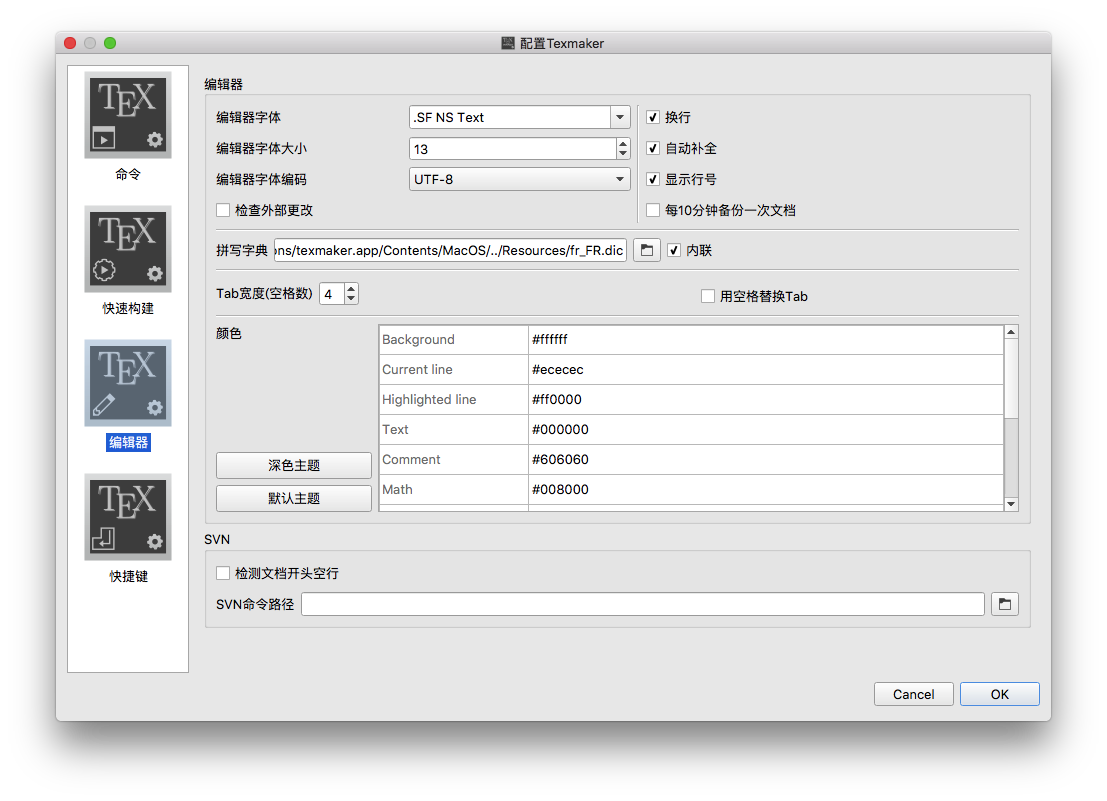
\includegraphics[width = 14cm]{Figure_05.png}
\caption{Texmaker 编辑器框中编辑器字体编码的设置}
\end{figure}

\item \doublebox{建立} 一个新文档,将以下代码 \doublebox{复制} 进入文档中,\doublebox{保存}。\\

\begin{lstlisting}
\documentclass{article}
\begin{document}
hello, world
\end{document}
\end{lstlisting}

\item \doublebox{运行} 工具栏中的 \doublebox{快速构建} 选项,观察编辑结果(\textbf{Figure 6})。
\begin{figure}[hbtp]
\centering \fboxrule = 1.2pt \fboxsep = 0pt \fcolorbox{gray}{white}{

\includegraphics[width = 10cm]{Figure_06.jpg}}
\caption{第一个 \LaTeX 文档的编辑效果}
\end{figure}
\end{enumerate}

\vspace{-2em}

\subsection{解密第一个 \LaTeX 文档}

\subsubsection{\LaTeX 的命令与环境}

\vspace{-2em}

\textbf{\begin{itemize}
\item[•]\LaTeX 命令以反斜线 \ovalbox{\textbackslash{}} 开头,为以下两种形式之一:
\textnormal{\begin{itemize}
\item[-]{反斜线和后面的一串字母,如 \ovalbox{\textbackslash{}LaTeX}。它们以任意非字母符号(空格、数字、标点等)作为分隔符。}
\item[-]{反斜线和后面的一个非字母符号,如 \ovalbox{\textbackslash{}\$}。它们无需分隔符。}
\end{itemize}}
\item[•]\LaTeX 的命令和参数:
\textnormal{\begin{itemize}
\item[-]{大多数的 \LaTeX 命令是带一个或多个参数,每个参数用花括号 \ovalbox{\{} 和 \ovalbox{\}} 包裹。}
\item[-]{除此之外,\LaTeX 的花括号本身也起到\textbf{分组}的作用,可以将字体、格式等的更改限制在大括号范围之内。}
\item[-]{有些命令带一个或多个可选参数,以方括号 \ovalbox{[} 和 \ovalbox{]} 包裹。}
\item[-]{还有些命令在命令名称后可以带一个星号 \ovalbox{*} ,带星号和不带星号的命令效果有一定差异。}
\end{itemize}}
\item[•]\LaTeX 还引入了环境的用法,用以令一些效果在局部生效,或是生成特定的文档元素。\LaTeX 环境的用法为一对命令 \ovalbox{\textbackslash{}begin} 和 \ovalbox{\textbackslash{}end}:\\
\vspace{-1em}
\begin{tcolorbox}[sharp corners, colback = green!30, colframe = green!80!blue, leftrule = 3mm, sharp corners, rounded corners = west, width=\linewidth, fontupper=\footnotesize,]
\textnormal{\textbackslash{}begin\{<environment name>\}\{<arguments>\}\\
 …\\
\textbackslash{}end\{<environment name>\}}
\end{tcolorbox}
\vspace{-3em}
\textnormal{\begin{itemize}
\item[-]{\ovalbox{<environment name>} 为环境名,\ovalbox{\textbackslash{}begin} 和 \ovalbox{\textbackslash{}end} 中填写的环境名应当一致。}
\item[-]{\ovalbox{\textbackslash{}begin} 在 \ovalbox{<environment name>} 后可以带一个或多个参数,甚至可选参数。}
\item[-]{环境允许嵌套使用。}
\end{itemize}}
\end{itemize}}

\subsubsection{\LaTeX 源代码结构}

\begin{enumerate}
\item \LaTeX 源代码以一个 \ovalbox{\textbackslash documentclass} 命令作为开头,它规定了文档使用的\textbf{文档类}:\\
\vspace{-1em}
\begin{tcolorbox}[sharp corners, colback = green!30, colframe = green!80!blue, leftrule = 3mm, sharp corners, rounded corners = west, width=\linewidth, fontupper=\footnotesize,]
\textbackslash documentclass\{ \ovalbox{article} / \ovalbox{report} / \ovalbox{book} / \ovalbox{slides} / \ovalbox{beamer} / \ovalbox{lettre} / \ovalbox{memoir} / \ovalbox{seminar} / … \}
\end{tcolorbox}
\vspace{-1em}
\item 接着 \ovalbox{\textbackslash documentclass} 命令之后,可以用 \ovalbox{\textbackslash usepackage} 命令调用宏包:\\
\vspace{-1em}
\begin{tcolorbox}[sharp corners, colback = green!30, colframe = green!80!blue, leftrule = 3mm, sharp corners, rounded corners = west, width=\linewidth, fontupper=\footnotesize,]
\textbackslash usepackage\{ \ovalbox{geometry} / \ovalbox{setspace} / \ovalbox{hyperref} / \ovalbox{xeCJK} / \ovalbox{enumitem} / \ovalbox{listings} / \ovalbox{tcolorbox} / … \}
\end{tcolorbox}
\vspace{-1em}
\item 最后,需要用以下一对命令来标记正文内容的开始位置和结束位置,从而将正文内容写入其中:\\
\vspace{-1em}
\begin{tcolorbox}[sharp corners, colback = green!30, colframe = green!80!blue, leftrule = 3mm, sharp corners, rounded corners = west, width=\linewidth, fontupper=\footnotesize,]
\textbackslash begin\{document\}\\
…\\
\textbackslash end\{document\}
\end{tcolorbox}
\end{enumerate}

\vspace{-1em}

\noindent
\textbf{注意}:在 \ovalbox{\textbackslash documentclass} 和 \ovalbox{\textbackslash begin\{document\}} 之间的位置称为\textbf{导言区},除了使用 \ovalbox{\textbackslash usepackage} 调用宏包之外,一些对文档的全局设置命令也在这里使用。当然也可以视自己的需求,什么都不写,一个宏包都不调用。

\section{了解 \LaTeX 的第二步}

\subsection{给文档添加标题、作者和注释}

\begin{enumerate}
\item \doublebox{建立} 一个新文档,将以下代码 \doublebox{复制} 进入文档中,\doublebox{保存}。\\
	
\begin{lstlisting}
\documentclass{article}
\author{My Name}
\title{The Title}
\begin{document}
\maketitle
hello, world % This is comment
\end{document}
\end{lstlisting}

\vspace{-2em}
	
\item \doublebox{运行} 工具栏中的 \doublebox{快速构建} 选项,观察编辑结果(\textbf{Figure 7})。
\begin{figure}[hbtp]
\centering \fboxrule = 1.2pt \fboxsep = 0pt \fcolorbox{gray}{white}{
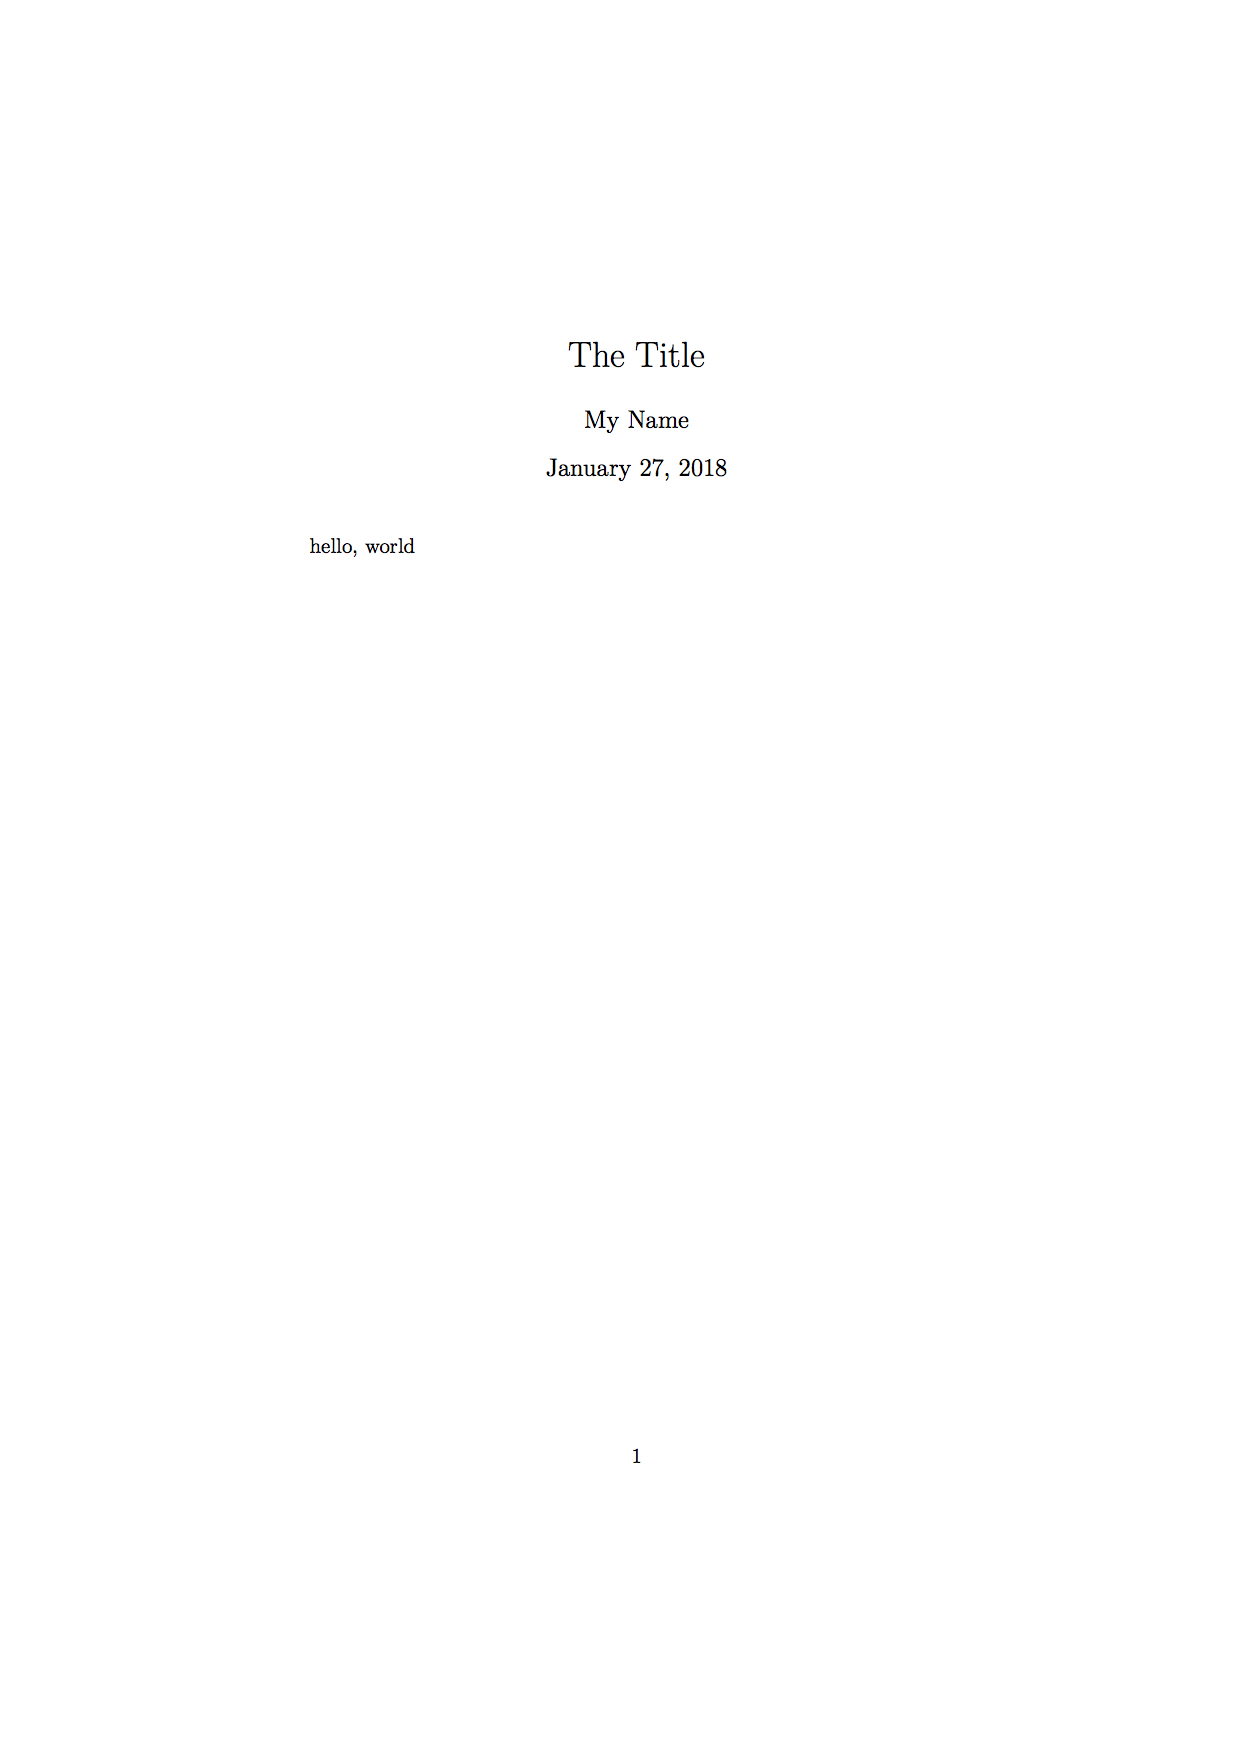
\includegraphics[width = 10cm]{Figure_07.jpg}}
\caption{\LaTeX 文档添加标题、作者和注释后的编辑效果}
\end{figure}
\end{enumerate}

\vspace{-2em}

\subsection{\LaTeX 的标题页和注释的添加方法}

\subsubsection{\LaTeX 的标题页}

\LaTeX 支持生成简单的标题页。首先需要给定标题和作者等信息:\\

\vspace{-1em}

\begin{tcolorbox}[sharp corners, colback = green!30, colframe = green!80!blue, leftrule = 3mm, sharp corners, rounded corners = west, width=\linewidth, fontupper=\footnotesize,]
\textbackslash title\{<title>\}\\
\textbackslash author\{<author>\}\\ 
\textbackslash date\{<date>\}
\end{tcolorbox}

其中前两个命令是必须的,\ovalbox{\textbackslash date} 命令可选。\LaTeX 还提供了一个 \ovalbox{\textbackslash today} 命令自动生成当前日期,可用在 \ovalbox{\textbackslash date} 的参数里,或者别的地方。\par
在 \ovalbox{\textbackslash title}、\ovalbox{\textbackslash author} 等命令内可以使用 \ovalbox{\textbackslash thanks} 命令生成标题页的脚注,如:\\

\vspace{-1em}

\begin{tcolorbox}[sharp corners, colback = green!30, colframe = green!80!blue, leftrule = 3mm, sharp corners, rounded corners = west, width=\linewidth, fontupper=\footnotesize,]
\textbackslash author\{Mary\textbackslash thanks\{E-mail:*****@***.com\}\}
\end{tcolorbox}

在信息给定后,就可以使用 \ovalbox{\textbackslash maketitle} 生成一个简单的标题页了。\ovalbox{article} 文档类的标题默认不单独成页,而 \ovalbox{report} 和 \ovalbox{book} 默认单独成 页。可在 \ovalbox{\textbackslash documentclass} 命令中指定 \ovalbox{titlepage / notitlepage} 选项修改。\par

\subsubsection{\LaTeX 的注释}
在科技著作的手稿中经常可以看到在边空里,在行间空白处,密密麻麻地写了很多文字,其中有些内容是遗漏补充,需要加入正文,有些则是注释,如对文稿中某些论述的说明、出处或考证等,这些注释内容通常不进入正文,专供作者备忘。在 \LaTeX 源文件中,可在任何位置使用注释标记,将上述这些注释内容完整地保留下来,以备作者查阅,而在编译后的PDF文件中还看不到这些注释内容。\par
在写作或者修改论文时,有时会将某些语句、段落或者图表公式等全部或部分删除,可事后又觉得不妥,但很难 恢复,只好重新再写。在 \LaTeX 中,可以利用注释的方法将这些需要删除的内容或可能会用到的资料保存下来,以备不时之需。科研论文要经过反复推敲,多次修改,注释功能非常实用。\par

\LaTeX 中的 \ovalbox{\%} 符号是注释符,它表示其右侧的文字是对左侧命令或文本的说明;在编译源文件时, \LaTeX 将忽略注释符及其右侧的所有字符。

\section{了解 \LaTeX 的第三步}

\subsection{结构化 \LaTeX 文档的实现}

\begin{enumerate}
\item \doublebox{建立} 一个新文档,将以下代码 \doublebox{复制} 进入文档中,\doublebox{保存}。\\

\begin{lstlisting}
\documentclass{article}
\title{Hello World}
\begin{document}
\maketitle
\section{Hello China} China is in East Asia.
\subsection{Hello Beijing} Beijing is the capital of China.
\subsubsection{Hello Dongcheng District}
\paragraph{Tian'anmen Square}is in the center of Beijing
\subparagraph{Chairman Mao} is in the center of Tian'anmen Square
\subsection{Hello Guangzhou}
\paragraph{Sun Yat-sen University} is the best university in Guangzhou.
\end{document}
\end{lstlisting}

\vspace{-2em}

\item \doublebox{运行} 工具栏中的 \doublebox{快速构建} 选项,观察编辑结果(\textbf{Figure 8})。
\begin{figure}[hbtp]
\centering \fboxrule = 1.2pt \fboxsep = 0pt \fcolorbox{gray}{white}{
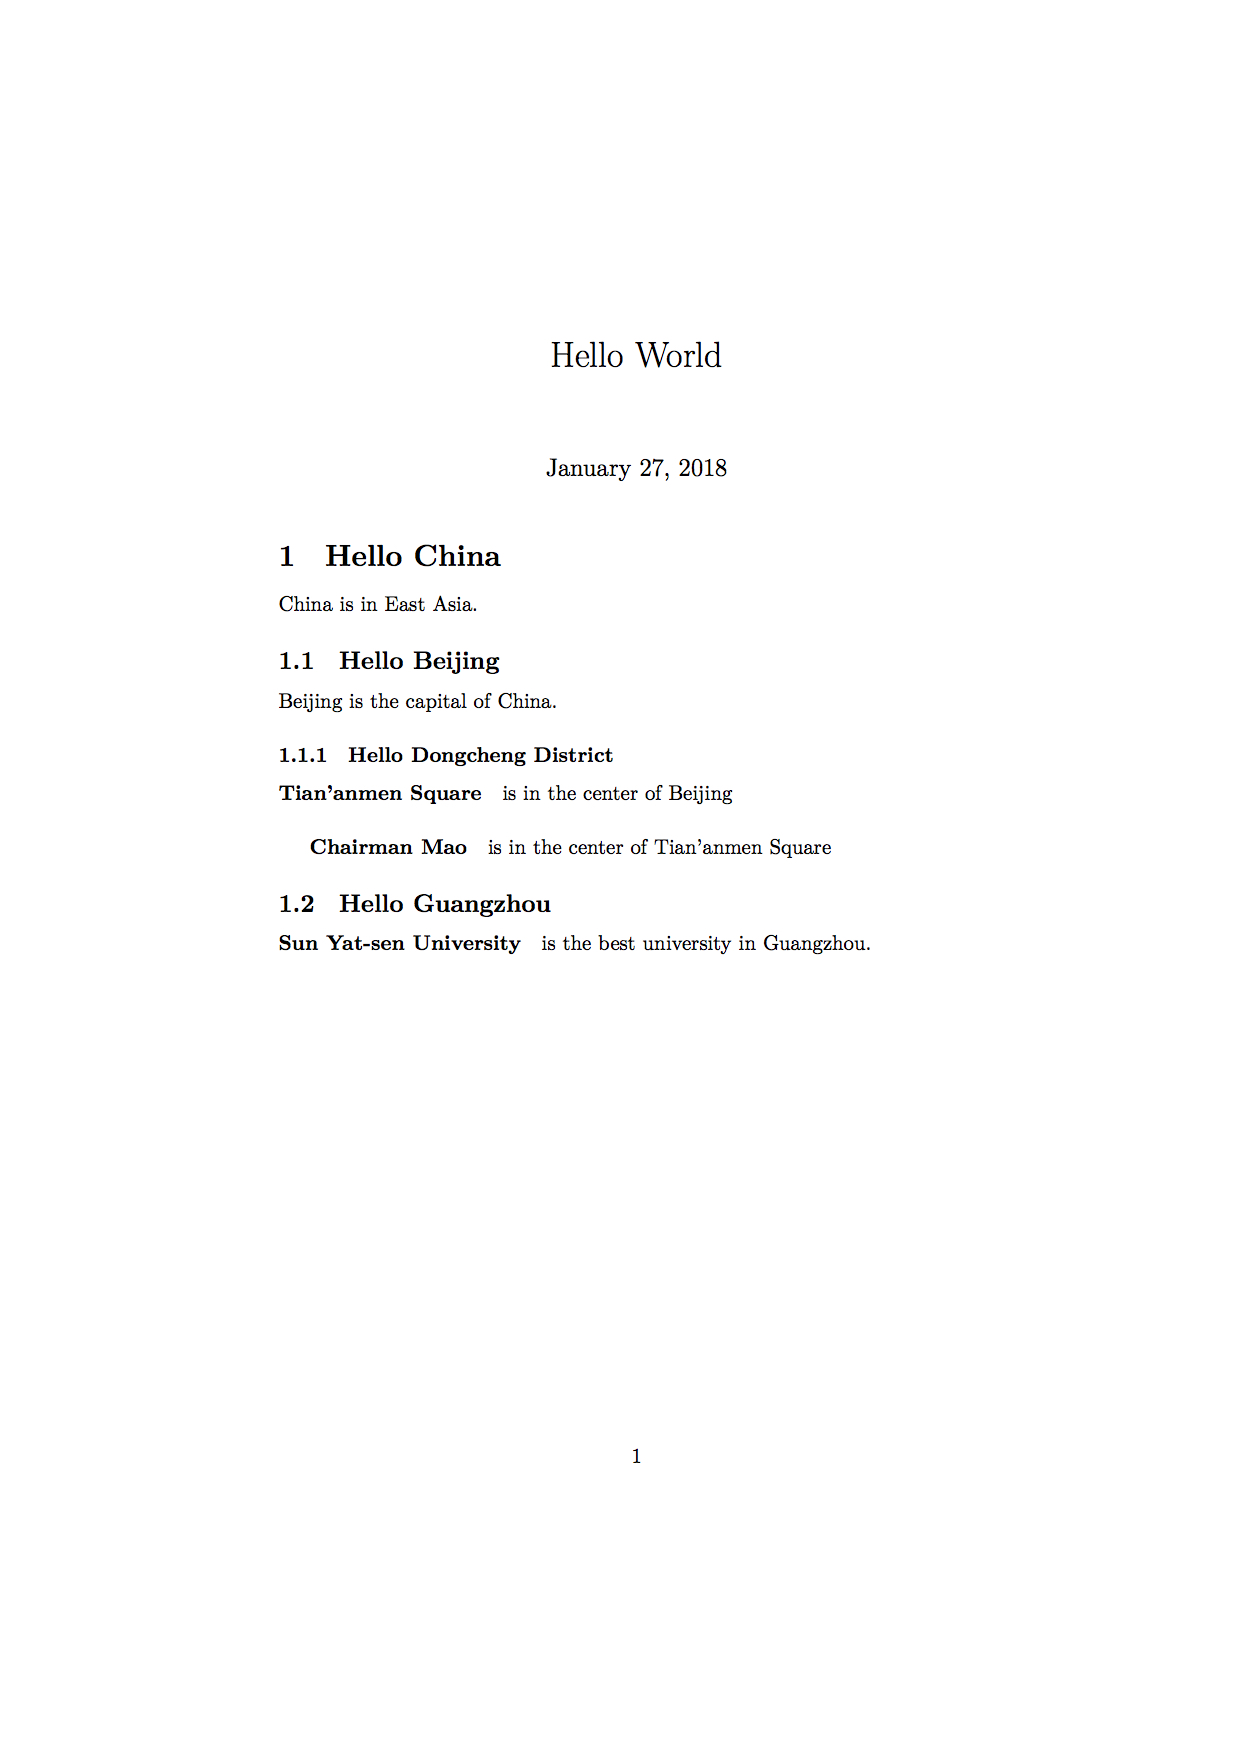
\includegraphics[width = 10cm]{Figure_08.jpg}}
\caption{结构化 \LaTeX 文档的编辑效果}
\end{figure}
\end{enumerate}

\vspace{-2em}

\subsection{区分 \LaTeX 章节和段落的方法}

\vspace{-2em}

\textbf{\begin{itemize}
\item[•]一篇结构化且条理清晰的文档一定是层次分明的,通过不同的命令分割为章、节、小节:
\textnormal{\begin{itemize}
\item[-]{\LaTeX 的三个\textbf{标准文档类} \ovalbox{article}、\ovalbox{report} 和 \ovalbox{book} 提供了一系列命令,用以划分章节、生成章节标题并自动编号:}
\begin{tcolorbox}[sharp corners, colback = green!30, colframe = green!80!blue, leftrule = 3mm, sharp corners, rounded corners = west, width=\linewidth, fontupper=\footnotesize,]
\textbackslash section\{<title>\}\quad
\textbackslash subsection\{<title>\}\quad
\textbackslash subsubsection\{<title>\}\quad
\textbackslash paragraph\{<title>\}\quad
\textbackslash subparagraph\{<title>\}
\end{tcolorbox}
\item[-]{\ovalbox{\textbackslash part} 命令用以将整个文档分割为大的分块,但不影响 \ovalbox{\textbackslash section} 等的编号:}
\begin{tcolorbox}[sharp corners, colback = green!30, colframe = green!80!blue, leftrule = 3mm, sharp corners, rounded corners = west, width=\linewidth, fontupper=\footnotesize,]
\textbackslash part\{<title>\}
\end{tcolorbox}
\item[-]{\ovalbox{book} 和 \ovalbox{report} 提供了章一级的结构:}
\begin{tcolorbox}[sharp corners, colback = green!30, colframe = green!80!blue, leftrule = 3mm, sharp corners, rounded corners = west, width=\linewidth, fontupper=\footnotesize,]
\textbackslash chapter\{<title>\}
\end{tcolorbox}
\end{itemize}}
\item[•]上述命令除了生成带编号的标题之外,还向目录中添加条目,并影响页眉页脚的内容。每个命令有两种变体:
\textnormal{\begin{itemize}
\item[-]{带可选参数的变体:}
\begin{tcolorbox}[sharp corners, colback = green!30, colframe = green!80!blue, leftrule = 3mm, sharp corners, rounded corners = west, width=\linewidth, fontupper=\footnotesize,]
\textbackslash section[<short title>]\{<title>\}\\
\textnormal{\textbf{此时}:标题使用 \ovalbox{<title>} 参数,在目录和页眉页脚中使用 \ovalbox{<short title>} 参数。}
\end{tcolorbox}
\item[-]{带星号的变体:}
\begin{tcolorbox}[sharp corners, colback = green!30, colframe = green!80!blue, leftrule = 3mm, sharp corners, rounded corners = west, width=\linewidth, fontupper=\footnotesize,]
\textbackslash section*\{<title>\}\\
\textnormal{\textbf{此时}:标题不带编号,也不生成目录项和页眉页脚。}
\end{tcolorbox}	
\end{itemize}}
\end{itemize}}

\vspace{-1em}

\noindent
\textbf{注意}:\LaTeX 并未提供为 \ovalbox{\textbackslash section} 等章节命令定制格式的功能,这一功能由 \ovalbox{titlesec} 宏包提供。

\section{了解 \LaTeX 的第四步}

\subsection{实现在 \LaTeX 中生成目录}

\begin{enumerate}
\item \doublebox{建立} 一个新文档,将以下代码 \doublebox{复制} 进入文档中,\doublebox{保存}。\\
	
\begin{lstlisting}
\documentclass{article}
\begin{document}
\tableofcontents
\section{Hello China} China is in East Asia.
\subsection{Hello Beijing} Beijing is the capital of China.
\subsubsection{Hello Dongcheng District}
\paragraph{Hello Tian'anmen Square}is in the center of Beijing
\subparagraph{Hello Chairman Mao} is in the center of Tian'anmen Square
\end{document}
\end{lstlisting}
	
\vspace{-2em}
	
\item \doublebox{运行} 工具栏中的 \doublebox{快速构建} 选项,观察编辑结果(\textbf{Figure 9})。
\begin{figure}[hbtp]
\centering \fboxrule = 1.2pt \fboxsep = 0pt \fcolorbox{gray}{white}{
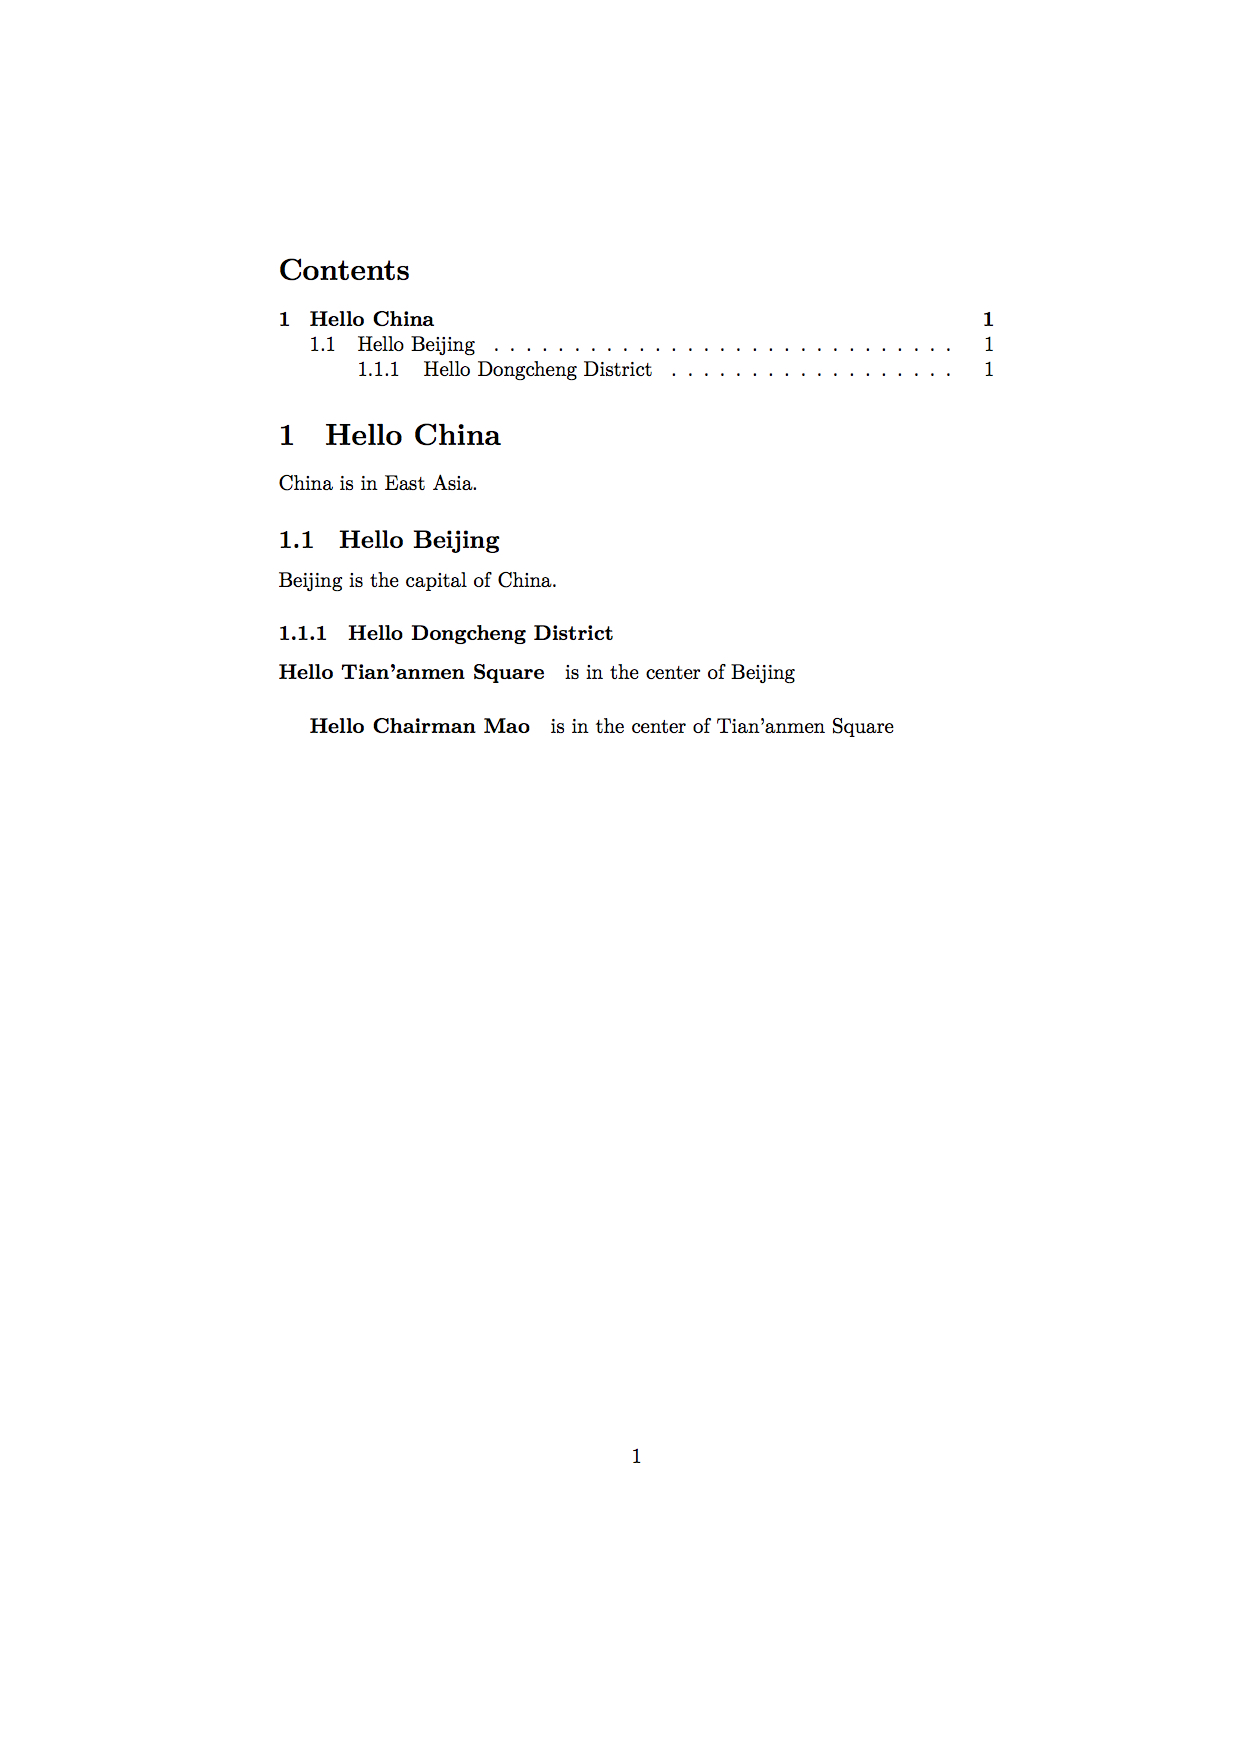
\includegraphics[width = 10cm]{Figure_09.jpg}}
\caption{\LaTeX 文档添加目录后的编辑效果}
\end{figure}
\end{enumerate}

\vspace{-2em}

\subsection{向 \LaTeX 文档加入目录的方法}

在 \LaTeX 中生成目录非常容易,只需在合适的地方使用命令:

\begin{tcolorbox}[sharp corners, colback = green!30, colframe = green!80!blue, leftrule = 3mm, sharp corners, rounded corners = west, width=\linewidth, fontupper=\footnotesize,]
\textbackslash tableofcontents
\end{tcolorbox}

正确生成目录项,一般需要多次编译源代码。
可以使用 \ovalbox{\textbackslash chapter*} 或 \ovalbox{\textbackslash section*} 这样不生成目录项的命令。\par

如果之后又想手动生成该章节的目录,可以在标题命令后面使用:

\begin{tcolorbox}[sharp corners, colback = green!30, colframe = green!80!blue, leftrule = 3mm, sharp corners, rounded corners = west, width=\linewidth, fontupper=\footnotesize,]
\textbackslash addcontentsline\{toc\}\{<level>\}\{<title>\}
\end{tcolorbox}

其中 \ovalbox{<level>} 为章节层次 \ovalbox{chapter} 或 \ovalbox{section} 等,\ovalbox{<title>} 为需要生成目录项的章节标题。

\section{了解 \LaTeX 的第五步}

\subsection{\LaTeX 文档换行的实现}

\begin{enumerate}
\item \doublebox{建立} 一个新文档,将以下代码 \doublebox{复制} 进入文档中,\doublebox{保存}。\\
	
\begin{lstlisting}
\documentclass{article}
\begin{document}
Beijing is
the capital
of China.

New York is

the capital

of America.

Amsterdam is \\ the capital \\
of Netherlands.
\end{document}
\end{lstlisting}
	
\vspace{-2em}
	
\item \doublebox{运行} 工具栏中的 \doublebox{快速构建} 选项,观察编辑结果(\textbf{Figure 10})。
\begin{figure}[hbtp]
\centering \fboxrule = 1.2pt \fboxsep = 0pt \fcolorbox{gray}{white}{
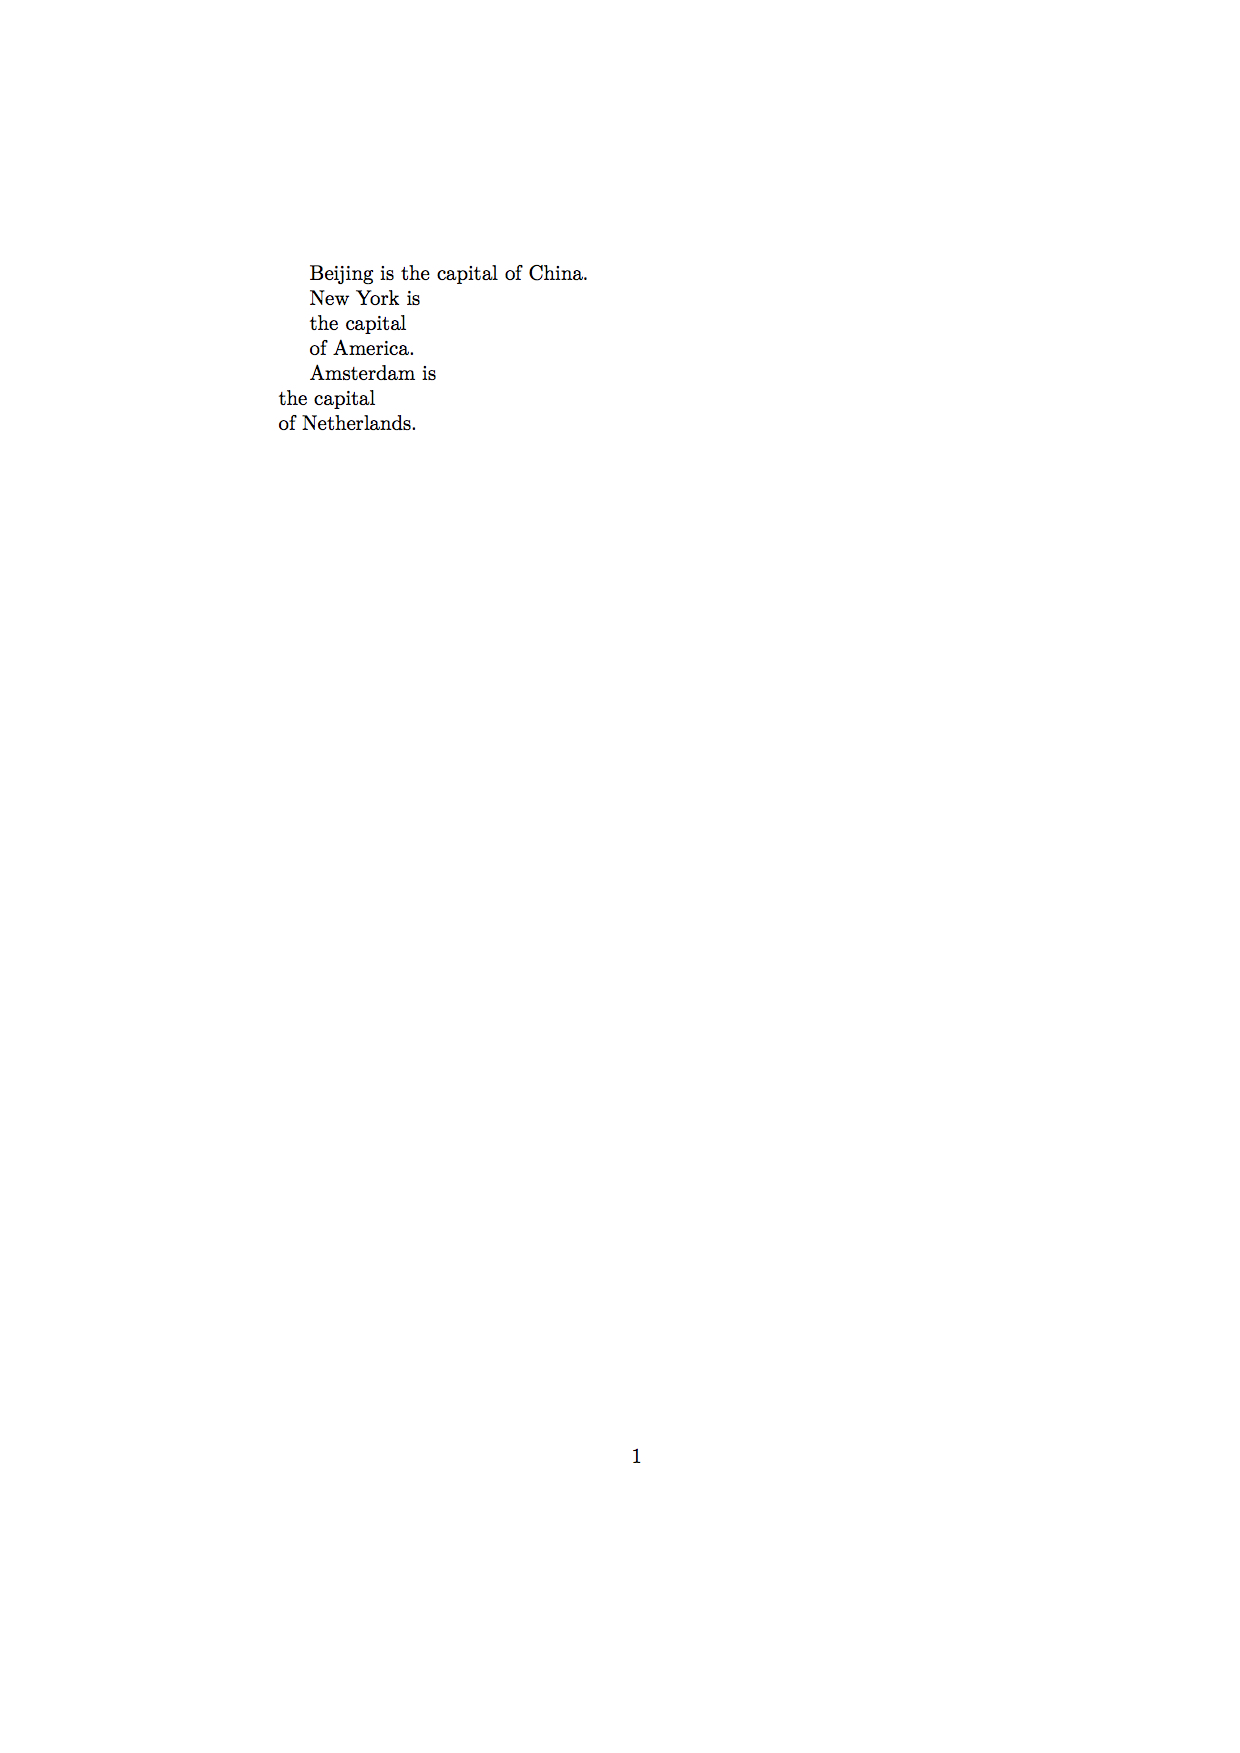
\includegraphics[width = 10cm]{Figure_10.jpg}}
\caption{不同 \LaTeX 文档换行方法的编辑效果}
\end{figure}
\end{enumerate}

\vspace{-2em}

\subsection{令 \LaTeX 文档立即换行的方法}

源文件经过编译后生成 PDF 格式文件,其行宽是由导言中版面尺寸命令或版面设置宏包设定的。因此,系统会根据所设定的版心宽度,即文本行的宽度,自动进行换行,必要时还可按照所设定的断词规则,在换行处自动进行断词处理,所以通常无须干预系统的自动换行工作。但有时根据某些情况或是某种环境要求,还是需要人为进行换行或者禁止换行处理。\par

如果由于某种原因需要在某处中断排版另起一行,可在该处插入换行命令:

\begin{tcolorbox}[sharp corners, colback = green!30, colframe = green!80!blue, leftrule = 3mm, sharp corners, rounded corners = west, width=\linewidth, fontupper=\footnotesize,]
\textbackslash \textbackslash \quad
\textbackslash \textbackslash *\quad
\textbackslash \textbackslash [高度]\quad
\textbackslash newline
\end{tcolorbox}		

系统将在此处结束当前行的排版并新起一行。其中:

\vspace{-4em}

\textbf{\begin{itemize}
\item[]		
\textnormal{\begin{itemize}		
\item[•]{命令 \ovalbox{\textbackslash \textbackslash} 表示在此换行。}
\item[•]而命令 \ovalbox{\textbackslash \textbackslash *} 表示在此换行,但是不能在此换页。
\item[•]命令 \ovalbox{\textbackslash \textbackslash [高度]} 表示在此换行,并且在当前行与下一行之间增加一段高度为此处所要求的高度的垂直空白,高度通常为正值,也可根据需要取负值,该命令多用于调节表格数据行之间的间隔,或多行公式之间的间隔。
\item[•]命令 \ovalbox{\textbackslash newline} 只能用于段落模式,而其他 3 种命令还可在某些数学环境中使用。
\end{itemize}}
\end{itemize}}

\noindent
\textbf{注意}:\LaTeX 源代码中,空格键和 Tab 键输入的空白字符视为\ovalbox{空格}。连续的若干个空白字符视为\ovalbox{一个空格}。每行开头的空格忽略不计。\par

\noindent
\textbf{注意}:行末的回车视为\ovalbox{一个空格};但连续两个回车,也就是\ovalbox{空行},会将文字分段。多个空行被视为\ovalbox{一个空行}。也可以在行末使用 \ovalbox{\textbackslash par} 命令\ovalbox{分段}。

\section{了解 \LaTeX 的第六步}

\subsection{使用 \LaTeX 实现数学公式的编辑}

\begin{enumerate}
\item \doublebox{建立} 一个新文档,将以下代码 \doublebox{复制} 进入文档中,\doublebox{保存}。\\
	
\begin{lstlisting}
\documentclass{article}
\usepackage{amsmath}
\usepackage{amssymb}
\begin{document}
The Newton's second law is F=ma.

The Newton's second law is $F=ma$.

The Newton's second law is
$$F=ma$$

The Newton's second law is
\[F=ma\]

Greek Letters $\eta$ and $\mu$

Fraction $\frac{a}{b}$

Power $a^b$

Subscript $a_b$

Derivate $\frac{\partial y}{\partial t} $

Vector $\vec{n}$

Bold $\mathbf{n}$

To time differential $\dot{F}$

Matrix (lcr here means left, center or right for each column)
\[
\left[
\begin{array}{lcr}
a1 & b22 & c333 \\
d444 & e555555 & f6
\end{array}
\right]
\]

Equations(here \& is the symbol for aligning different rows)
\begin{align}
a+b&=c\\
d&=e+f+g
\end{align}

\[
\left\{
\begin{aligned}
&a+b=c\\
&d=e+f+g
\end{aligned}
\right.
\]

\end{document}
\end{lstlisting}
	
\vspace{-2em}
	
\item \doublebox{运行} 工具栏中的 \doublebox{快速构建} 选项,观察编辑结果(\textbf{Figure 11})。
\begin{figure}[hbtp]
\centering \fboxrule = 1.2pt \fboxsep = 0pt \fcolorbox{gray}{white}{
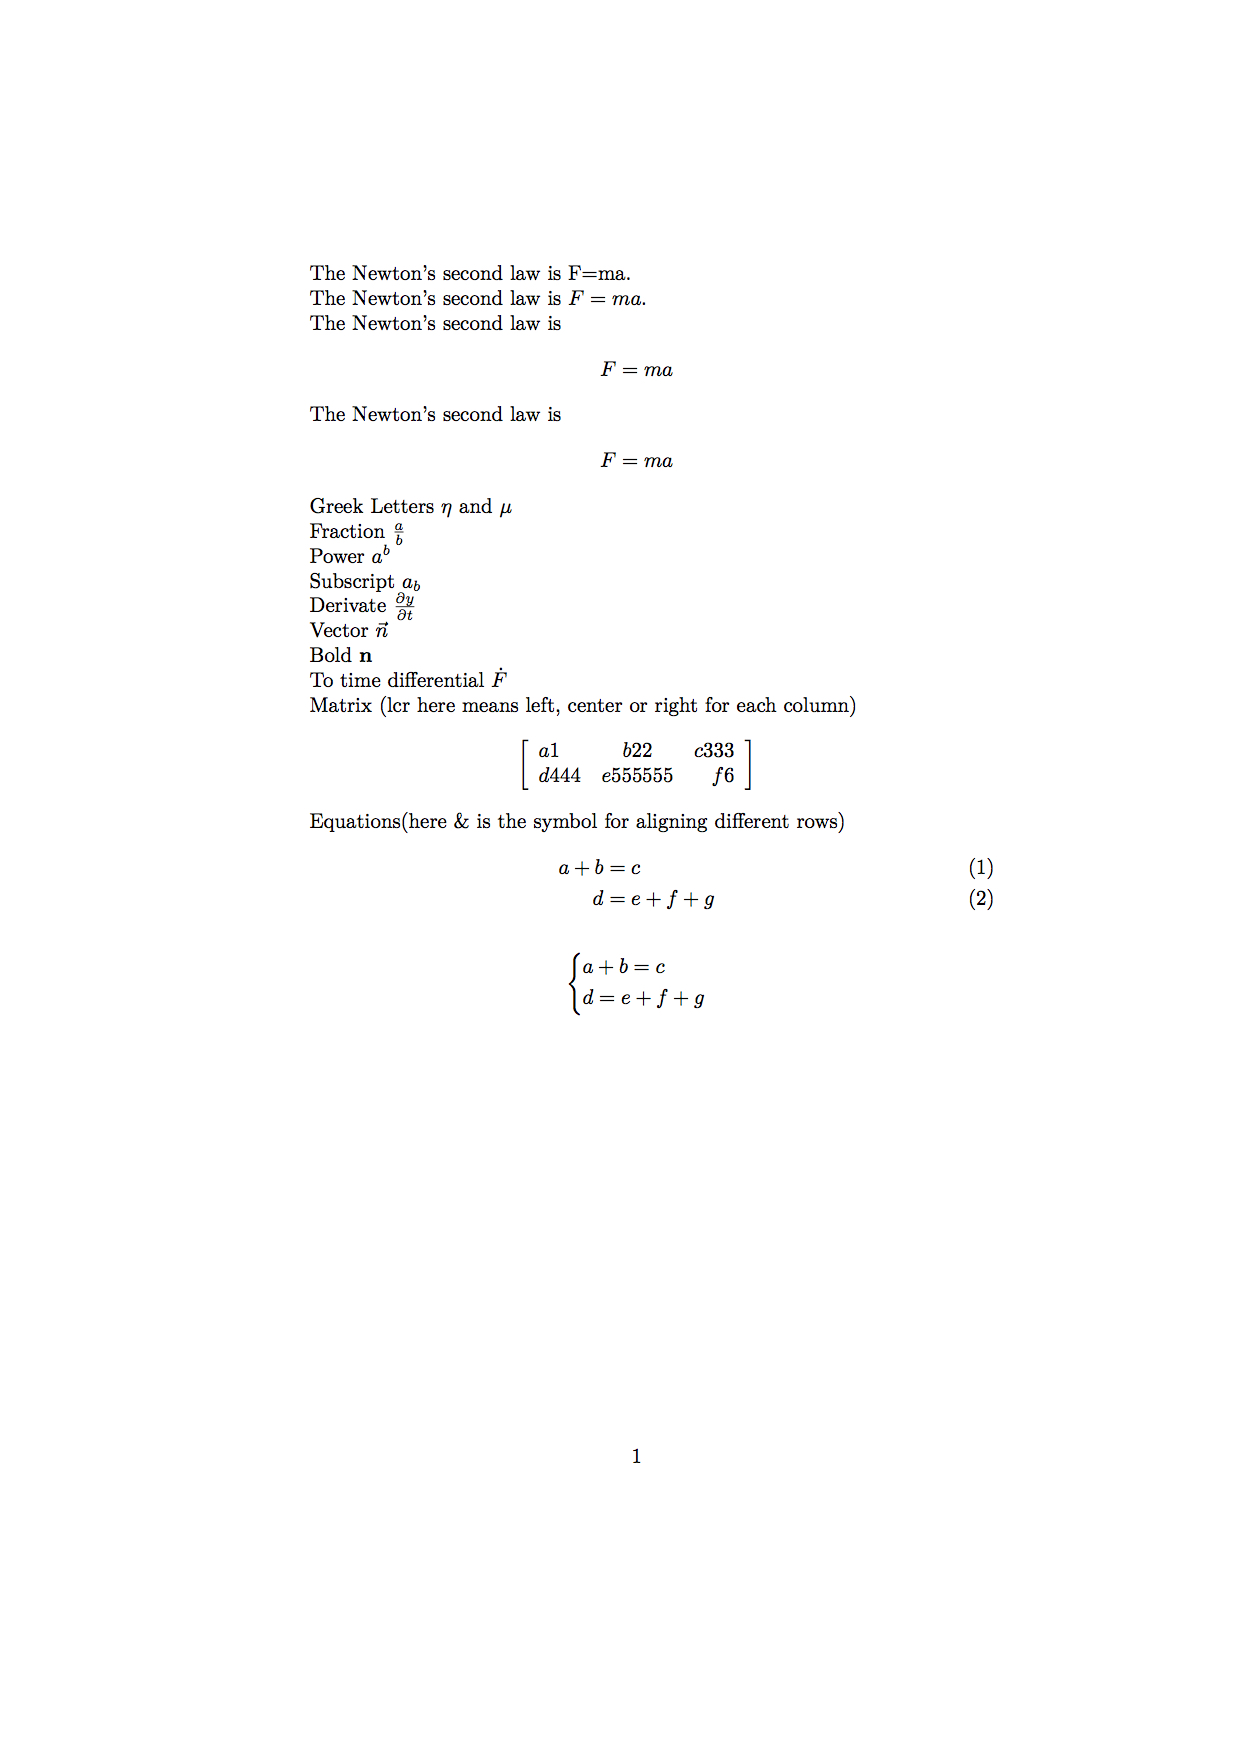
\includegraphics[width = 10cm]{Figure_11.jpg}}
\caption{\LaTeX 文档适用于各种简单或者复杂的数学公式}
\end{figure}
\end{enumerate}

\vspace{-2em}

\subsection{\hologo{AmSLaTeX} 宏集}

\hologo{AmSLaTeX} 宏集合是美国数学学会(\textit{American Mathematical Society})提供的对 \LaTeX 原生的数学公式排版的扩展,其核心是 \ovalbox{amsmath} \textbf{宏包},对多行公式的排版提供了有力的支持。此外,\ovalbox{amsfonts} \textbf{宏包}以及基于它的 \ovalbox{amssymb} \textbf{宏包}提供了丰富的数学符号;\ovalbox{amsthm} \textbf{宏包}扩展了 \LaTeX 定理证明格式。

\subsubsection{公式排版基础}

数学公式有两种排版方式:其一是与文字混排,称为\textbf{行内公式};其二是单独列为一行排版, 称为\textbf{行间公式}。\par

\textbf{行内公式}由一对 \ovalbox{\$} 符号包裹。

\begin{tcolorbox}[title = 行内公式,
colback = green!50!yellow!25!white,
colframe = green!80!blue,
colbacktitle = green!80!yellow!50!white,
coltitle = green!25!black,
fonttitle = \bfseries,
subtitle style = {boxrule = 1pt,
colback = green!30} ]
\LaTeX 可以将数学公式与文字混合排版,此方式称为\textbf{行内公式}。
\tcbsubtitle{执行代码}
Add \$a\$ squared and \$b\$ squared
to get \$c\$ squared. Or, using
a more mathematical approach:
\$a\textasciicircum{}2 + b\textasciicircum{}2 = c\textasciicircum{}2\$
\tcbsubtitle{执行效果}
Add $a$ squared and $b$ squared
to get $c$ squared. Or, using
a more mathematical approach:
$a^2 + b^2 = c^2$
\end{tcolorbox}

单独成行的\textbf{行间公式}在 \LaTeX 里由 \ovalbox{equation} 环境包裹。\ovalbox{equation} 环境为公式自动生成一个编号,这个编号可以用 \ovalbox{\textbackslash label} 和 \ovalbox{\textbackslash ref} 生成交叉引用,\ovalbox{amsmath} 的\ovalbox{\textbackslash eqref} 命令甚至为引用自动加上圆括号;还可以用 \ovalbox{\textbackslash tag} 命令手动修改公式的编号,或者用 \ovalbox{\textbackslash notag} 命令取消为公式编号(与之基本等效的命令是 \ovalbox{\textbackslash nonumber})。

\begin{tcolorbox}[title = 行间公式,
colback = green!50!yellow!25!white,
colframe = green!80!blue,
colbacktitle = green!80!yellow!50!white,
coltitle = green!25!black,
fonttitle = \bfseries,
subtitle style = {boxrule = 1pt,
colback = green!30} ]
\LaTeX 也可以将数学公式以单独列为一行的方式来排版,此方式称为\textbf{行间公式}。
\tcbsubtitle{执行代码}
Add \$a\$ squared and \$b\$ squared
to get \$c\$ squared\\
\textbackslash begin\{equation\}\\
a\textasciicircum{}2 + b\textasciicircum{}2 = c\textasciicircum{}2\\
\textbackslash end\{equation\}\\
Einstein says\\
\textbackslash begin\{equation\}\\
E = mc\textasciicircum{}2 \textbackslash label\{clever\}\\
\textbackslash end\{equation\}\\
This is a reference to
\textbackslash eqref\{clever\}.
\tcbsubtitle{执行效果}
Add $a$ squared and $b$ squared
to get $c$ squared
\begin{equation}
a^2 + b^2 = c^2
\end{equation}
Einstein says
\begin{equation}
E = mc^2 \label{clever}
\end{equation}
This is a reference to
\eqref{clever}.
\end{tcolorbox}

\begin{tcolorbox}[title = 执行代码,
colback = green!50!yellow!25!white,
colframe = green!80!blue,
colbacktitle = green!30,
coltitle = green!25!black,
fonttitle = \bfseries]
It’s wrong to say\\
\textbackslash begin\{equation\}\\
1 + 1 = 3 \textbackslash tag\{dumb\}\\
\textbackslash end\{equation\}\\
or\\
\textbackslash begin\{equation\}\\
1 + 1 = 4 \textbackslash notag\\
\textbackslash end\{equation\}
\tcbsubtitle{执行效果}
It’s wrong to say
\begin{equation}
1 + 1 = 3 \tag{dumb}
\end{equation}
or
\begin{equation}
1 + 1 = 4 \notag
\end{equation}
\end{tcolorbox}

除了可以为每个公式手动取消编号,\LaTeX 提供了一对命令 \ovalbox{\textbackslash [} 和 \ovalbox{\textbackslash ]} 用于生成不带编号的行间公式,与之等效的是 \ovalbox{displaymath} 环境和 \ovalbox{equation*} 环境。行间公式是否有带编号,体现了带星号的 \ovalbox{equation*} 环境和不带星号的\ovalbox{equation} 环境之间的区别。

\begin{tcolorbox}[title = 执行代码,
colback = green!50!yellow!25!white,
colframe = green!80!blue,
colbacktitle = green!30,
coltitle = green!25!black,
fonttitle = \bfseries]
Again\textbackslash{}ldots\\
\textbackslash{}begin\{equation*\}\\
a\textasciicircum{}2 + b\textasciicircum{}2 = c\textasciicircum{}2\\
\textbackslash{}end\{equation*\}\\
or you can type less for the same effect:
\textbackslash{}[ a\textasciicircum{}2 + b\textasciicircum{}2 = c\textasciicircum{}2 \textbackslash{}]\\
or if you like the long one:\\
\textbackslash{}begin\{displaymath\}\\
a\textasciicircum{}2 + b\textasciicircum{}2 = c\textasciicircum{}2\\
\textbackslash{}end\{displaymath\}
\tcbsubtitle{执行效果}
Again\ldots
\begin{equation*}
a^2 + b^2 = c^2
\end{equation*}
or you can type less for the
same effect:
\[ a^2 + b^2 = c^2 \]
or if you like the long one:
\begin{displaymath}
a^2 + b^2 = c^2
\end{displaymath}
\end{tcolorbox}

\TeX 原生排版行间公式的方法是用一对 \ovalbox{\$\$} 符号包裹,不过无法通过指定 \ovalbox{fleqn} 选项控制左对齐,与上下文之间的间距也不好调整,故不太推荐使用。\par

行间公式的对齐、编号位置等性质由文档类选项控制,文档类的 \ovalbox{fleqn} 选项令行间公式左对齐;\ovalbox{leqno} 选项令编号放在公式左边。\par

\vspace{1em}

\noindent
\textbf{注意}:对比 \LaTeX 的行内公式与行间公式,由于行内公式为了与文字相适应,其在排版大的公式元素(分式、巨算符等)时显得很“局促”。

\subsubsection{数学模式和文本}

当使用 \$ 开启行内公式输入,或是使用 \ovalbox{\textbackslash{}[} 命令、\ovalbox{equation} 环境时,便进入了所谓的\textbf{数学模式}。\textbf{数学模式}相比于文本模式有以下\textbf{特点}:

\begin{enumerate}
\item 数学模式中输入的空格全部被忽略。数学符号的间隙默认完全由符号的性质(关系符号、运算符等)决定。需要人为引入空隙时,使用 \ovalbox{\textbackslash{}quad} 和 \ovalbox{\textbackslash{}qquad} 等命令。
\item \textbf{不允许有空行(分段)。}每个公式(每组多行公式)自成一个段落。
\item 所有的字母被当作数学公式中的变量处理,字母间距与文本模式不一致,也无法生成单词之间的空格。如果想在数学公式中输入正体的文本,简单情况下可用 \ovalbox{\textbackslash{}mathrm} 命令。\ovalbox{\textbackslash{}amsmath} 提供了更加方便的 \ovalbox{\textbackslash{}text} 命令。
\end{enumerate}

\begin{tcolorbox}[title = 执行代码,
colback = green!50!yellow!25!white,
colframe = green!80!blue,
colbacktitle = green!30,
coltitle = green!25!black,
fonttitle = \bfseries]
 \$x\textasciicircum{}\{2\} \textbackslash{}geq 0 \textbackslash{}qquad\\
\textbackslash{}text\{for \textbackslash{}textbf\{all\} \}\\
x\textbackslash{}in\textbackslash{}mathbb\{R\}\$
\tcbsubtitle{执行效果}
 $x^{2} \geq 0 \qquad
\text{for \textbf{all} }
x\in\mathbb{R}$
\end{tcolorbox}

\vspace{0.5em}

\noindent
\textbf{注意}:\ovalbox{\textbackslash{}text} 命令仅适合在公式中穿插少量文字。如果需要在许多文字中穿插使用公式,则应该像正常的行内公式那样,而不是滥用 \ovalbox{\textbackslash{}text} 命令。

\subsubsection{一般数学符号与上下标}

\vspace{-2em}

\textbf{\begin{itemize}
\item[•]一般符号
\textnormal{\begin{itemize}
\item[-]{小写希腊字母符:$\alpha$ \ovalbox{\textbackslash{}alpha}、$\beta$ \ovalbox{\textbackslash{}beta}、$\eta$ \ovalbox{\textbackslash{}eta}、$\mu$ \ovalbox{\textbackslash{}mu}}
\item[-]{大写希腊字母符(首字母大写):$\Gamma$ \ovalbox{\textbackslash{}Gamma}、$\Delta$ \ovalbox{\textbackslash{}Delta}}
\item[-]{无穷大符号:$\infty$ \ovalbox{\textbackslash{}infty}}
\item[-]{普通省略号,具有两种形式。\textbf{需要注意}的是,这两种形式的省略号有各自合适的用途。另外,\ovalbox{\textbackslash{}ldots} 和 \ovalbox{\textbackslash{}dots} 是完全等效的,它们既能用在公式中,也用来在文本里作为省略号。}
\begin{tcolorbox}[title = 执行代码,
colback = green!50!yellow!25!white,
colframe = green!80!blue,
colbacktitle = green!30,
coltitle = green!25!black,
fonttitle = \bfseries]
\$a\_1, a\_2, \textbackslash{}dots, a\_n\$ \textbackslash{}\textbackslash{}\\
\$a\_1 + a\_2 + \textbackslash{}cdots + a\_n\$
\tcbsubtitle{执行效果}
$a_1, a_2, \dots, a_n$ \\
$a_1 + a_2 + \cdots + a_n$
\end{tcolorbox}
\item[-]{矩阵中会用到的竖排或斜排省略号:$\vdots$  \ovalbox{\textbackslash{}vdots}、$\ddots$ \ovalbox{\textbackslash{}ddots}}
\end{itemize}}
\item[•]指数、上下标和导数
\textnormal{\begin{itemize}
\item[-]{\LaTeX 用 \ovalbox{\textasciicircum{}} 和 \ovalbox{\_} 标明上、下标。\textbf{需要注意}的是,上、下标的内容(子公式)一般需要用花括号包裹,否则上、下标只对后面的第一个符号起作用。}
\begin{tcolorbox}[title = 执行代码,
colback = green!50!yellow!25!white,
colframe = green!80!blue,
colbacktitle = green!30,
coltitle = green!25!black,
fonttitle = \bfseries]
\$p\textasciicircum{}3\_\{ij\} \textbackslash{}qquad
m\_\textbackslash{}mathrm\{Knuth\}\textbackslash{}qquad
\textbackslash{}sum\_\{k=1\}\textasciicircum{}3 k \$\textbackslash{}\textbackslash{}[5pt]\\
\$a\textasciicircum{}x+y \textbackslash{}neq a\textasciicircum{}\{x+y\}\textbackslash{}qquad
e\textasciicircum{}\{x\textasciicircum{}2\} \textbackslash{}neq \{e\textasciicircum{}x\}\textasciicircum{}2\$
\tcbsubtitle{执行效果}
$p^3_{ij} \qquad
m_\mathrm{Knuth}\qquad
\sum_{k=1}^3 k $\\[5pt]
$a^x+y \neq a^{x+y}\qquad
e^{x^2} \neq {e^x}^2$
\end{tcolorbox}
\item[-]{导数符号 \ovalbox{$'$} 是一类特殊的上标,可以适当连用表示多阶导数,也可以在其后连用上标。}
\begin{tcolorbox}[title = 执行代码,
colback = green!50!yellow!25!white,
colframe = green!80!blue,
colbacktitle = green!30,
coltitle = green!25!black,
fonttitle = \bfseries]
\$f(x) = x\textasciicircum{}2 \textbackslash{}quad f$'$(x)
= 2x \textbackslash{}quad f$''$\textasciicircum{}\{2\}(x) = 4\$
\tcbsubtitle{执行效果}
$f(x) = x^2 \quad f'(x)
= 2x \quad f''^{2}(x) = 4$
\end{tcolorbox}
\end{itemize}}
\end{itemize}}

\subsubsection{分式和根式}
分式使用 \ovalbox{\textbackslash{}frac\{分子\}\{分母\}} 来书写。分式的大小在行间公式中是正常大小,而在行内被极度压缩。\ovalbox{amsmath} 提供了方便的命令 \ovalbox{\textbackslash{}dfrac} 和 \ovalbox{\textbackslash{}tfrac},令用户能够在行内使用正常大小的行间公式,或是反过来。

\begin{tcolorbox}[title = 执行代码,
colback = green!50!yellow!25!white,
colframe = green!80!blue,
colbacktitle = green!30,
coltitle = green!25!black,
fonttitle = \bfseries]
In display style:\\
\textbackslash{}[\\
3/8 \textbackslash{}qquad \textbackslash{}frac\{3\}\{8\}
\textbackslash{}qquad \textbackslash{}tfrac\{3\}\{8\}\\
\textbackslash{}]\\
In text style:\\
\$1\textbackslash{}frac\{1\}\{2\}\$\textasciitilde hours \textbackslash{}qquad\\
\$1\textbackslash{}dfrac\{1\}\{2\}\$\textasciitilde hours
\tcbsubtitle{执行效果}
In display style:
\[
3/8 \qquad \frac{3}{8}
\qquad \tfrac{3}{8}
\]\\
In text style:
$1\frac{1}{2}$~hours \qquad
$1\dfrac{1}{2}$~hours
\end{tcolorbox}

一般的根式使用 \ovalbox{\textbackslash{}sqrt\{\ldots\}};表示 $n$ 次方根时写成  \ovalbox{\textbackslash{}sqrt[n]\{\ldots\}}。

\begin{tcolorbox}[title = 执行代码,
colback = green!50!yellow!25!white,
colframe = green!80!blue,
colbacktitle = green!30,
coltitle = green!25!black,
fonttitle = \bfseries]
\$\textbackslash{}sqrt\{x\} \textbackslash{}Leftrightarrow x\textasciicircum{}\{1/2\}
\textbackslash{}quad \textbackslash{}sqrt[3]\{2\}
\textbackslash{}quad \textbackslash{}sqrt\{x\textasciicircum{}\{2\} + \textbackslash{}sqrt\{y\}\}\$
\tcbsubtitle{执行效果}
$\sqrt{x} \Leftrightarrow x^{1/2}
\quad \sqrt[3]{2}
\quad \sqrt{x^{2} + \sqrt{y}}$
\end{tcolorbox}

特殊的分式形式,如二项式结构,由 \ovalbox{amsmath} 宏包的 \ovalbox{\textbackslash{}binom} 命令生成。

\begin{tcolorbox}[title = 执行代码,
colback = green!50!yellow!25!white,
colframe = green!80!blue,
colbacktitle = green!30,
coltitle = green!25!black,
fonttitle = \bfseries]
 Pascal’s rule is\\
\textbackslash{}[\\
\textbackslash{}binom\{n\}\{k\} =\textbackslash{}binom\{n-1\}\{k\} + \textbackslash{}binom\{n-1\}\{k-1\}\\
\textbackslash{}]
\tcbsubtitle{执行效果}
 Pascal’s rule is
\[
\binom{n}{k} =\binom{n-1}{k} + \binom{n-1}{k-1}
\]
\end{tcolorbox}

\subsubsection{关系符与算符}

\LaTeX 常见的\textbf{关系符号}除了可以直接输入的 \ovalbox{\textbackslash{}=}、\ovalbox{\textbackslash{}>}、\ovalbox{\textbackslash{}<},其它符号用命令输入,常用的有不等号 $\ne$ \ovalbox{\textbackslash{}ne}、大于等于号 $\ge$ \ovalbox{\textbackslash{}ge} 和小于等于号 $\le$ \ovalbox{\textbackslash{}le}、约等号 $\approx$ \ovalbox{\textbackslash{}approx}、等价 $\equiv$ \ovalbox{\textbackslash{}equiv}、正比 $\propto$ \ovalbox{\textbackslash{}propto}、相似 $\sim$ \ovalbox{\textbackslash{}sim} 等等。此外,倾斜的关系符号 $\leqslant$ \ovalbox{\textbackslash{}leqslant} 和 $\geqslant$ \ovalbox{\textbackslash{}geqslant} 由 \ovalbox{amssymb} 提供。\par

\LaTeX 还提供了自定义二元关系符的命令 \ovalbox{\textbackslash{}stackrel},用于将一个符号叠加在原有的二元关系符之上。

\begin{tcolorbox}[title = 执行代码,
colback = green!50!yellow!25!white,
colframe = green!80!blue,
colbacktitle = green!30,
coltitle = green!25!black,
fonttitle = \bfseries]
\textbackslash{}[\\
f\_n(x) \textbackslash{}stackrel\{*\}\{\textbackslash{}approx\} 1\\
\textbackslash{}]
\tcbsubtitle{执行效果}
 \[
f_n(x) \stackrel{*}{\approx} 1
\]
\end{tcolorbox}

\LaTeX 中的\textbf{算符}大多数是\textbf{二元算符},除了直接用键盘可以输入的 \ovalbox{+}、\ovalbox{−}、\ovalbox{*}、\ovalbox{/},其它符号用命令输入,常用的有乘号 $\times$ \ovalbox{\textbackslash{}times}、除号 $\div$ \ovalbox{\textbackslash{}div}、点乘 $\cdot$ \ovalbox{\textbackslash{}cdot}、加减号 $\pm$ \ovalbox{\textbackslash{}pm} / $\mp$ \ovalbox{\textbackslash{}mp} 等等。\par

$\nabla$ \ovalbox{\textbackslash{}nabla} 和 $\partial$ \ovalbox{\textbackslash{}partial} 也是常用的算符,虽然它们不属于二元算符。\par

\LaTeX 将数学函数的名称作为一个算符排版,字体为直立字体。其中有一部分符号在上下位置可以书写一些内容作为条件,类似于\textbf{巨算符}。

\begin{tcolorbox}[title = 执行代码,
colback = green!50!yellow!25!white,
colframe = green!80!blue,
colbacktitle = green!30,
coltitle = green!25!black,
fonttitle = \bfseries]
\textbackslash{}[\\
\textbackslash{}lim\_\{x \textbackslash{}rightarrow 0\}
\textbackslash{}frac\{\textbackslash{}sin x\}\{x\}=1\\
\textbackslash{}]
\tcbsubtitle{执行效果}
\[
\lim_{x \rightarrow 0}
\frac{\sin x}{x}=1
\]
\end{tcolorbox}

对于求模表达式,\LaTeX 提供了 \ovalbox{\textbackslash{}pmod} 和 \ovalbox{\textbackslash{}bmod} 命令,前者相当于一个二元运算符,后者作为同余表达式的后缀。

\begin{tcolorbox}[title = 执行代码,
colback = green!50!yellow!25!white,
colframe = green!80!blue,
colbacktitle = green!30,
coltitle = green!25!black,
fonttitle = \bfseries]
\$a\textbackslash{}bmod b \textbackslash{}\textbackslash{}\\
x\textbackslash{}equiv a \textbackslash{}pmod\{b\}\$
\tcbsubtitle{执行效果}
$a\bmod b \\
x\equiv a \pmod{b}$
\end{tcolorbox}

此外,\ovalbox{amsmath} 允许用户用 \ovalbox{\textbackslash{}DeclareMathOperator} 定义自己的算符,其中带星号的命令定义带上下限的算符。

\begin{tcolorbox}[title = 导言区,
colback = green!50!yellow!25!white,
colframe = green!80!blue,
colbacktitle = green!80!yellow!50!white,
coltitle = green!25!black,
fonttitle = \bfseries,
subtitle style = {boxrule = 1pt,
colback = green!30} ]
\textbackslash{}DeclareMathOperator\{\textbackslash{}argh\}\{argh\}\\
\textbackslash{}DeclareMathOperator*\{\textbackslash{}nut\}\{Nut\}
\tcbsubtitle{执行代码}
\textbackslash{}[\textbackslash{}argh 3 = \textbackslash{}nut\_\{x=1\} 4x\textbackslash{}]
\tcbsubtitle{执行效果}
\[\argh 3 = \nut_{x=1} 4x\]
\end{tcolorbox}

\subsubsection{巨算符}
积分号 $\int$ \ovalbox{\textbackslash{}int}、求和号 $\sum$ \ovalbox{\textbackslash{}sum} 等符号称为\textbf{巨算符}。巨算符在行内公式和行间公式的大小和形状有区别。

\begin{tcolorbox}[title = 执行代码,
colback = green!50!yellow!25!white,
colframe = green!80!blue,
colbacktitle = green!30,
coltitle = green!25!black,
fonttitle = \bfseries]
In text:\\
\$\textbackslash{}sum\_\{i=1\}\textasciicircum{}n \textbackslash{}quad
\textbackslash{}int\_0\textasciicircum{}\{\textbackslash{}frac\{\textbackslash{}pi\}\{2\}\} \textbackslash{}quad
\textbackslash{}oint\_0\textasciicircum{}\{\textbackslash{}frac\{\textbackslash{}pi\}\{2\}\} \textbackslash{}quad
\textbackslash{}prod\_\textbackslash{}epsilon \$ \textbackslash{}\textbackslash{}\\
In display:\\
\textbackslash{}[\textbackslash{}sum\_\{i=1\}\textasciicircum{}n \textbackslash{}quad
\textbackslash{}int\_0\textasciicircum{}\{\textbackslash{}frac\{\textbackslash{}pi\}\{2\}\} \textbackslash{}quad
\textbackslash{}oint\_0\textasciicircum{}\{\textbackslash{}frac\{\textbackslash{}pi\}\{2\}\} \textbackslash{}quad
\textbackslash{}prod\_\textbackslash{}epsilon \textbackslash{}]
\tcbsubtitle{执行效果}
In text:
$\sum_{i=1}^n \quad
\int_0^{\frac{\pi}{2}} \quad
\oint_0^{\frac{\pi}{2}} \quad
\prod_\epsilon $ \\
In display:
\[\sum_{i=1}^n \quad
\int_0^{\frac{\pi}{2}} \quad
\oint_0^{\frac{\pi}{2}} \quad
\prod_\epsilon \]
\end{tcolorbox}

巨算符的上下标用作其上下限。\textbf{行间公式}中,积分号默认将上下限放在右上角和右下角,求和号默认在上下方;\textbf{行内公式}一律默认在右上角和右下角。可以在巨算符后使用 \ovalbox{\textbackslash{}limits} 手动令上下限显示在上下方,\ovalbox{\textbackslash{}nolimits} 则相反。

\begin{tcolorbox}[title = 执行代码,
colback = green!50!yellow!25!white,
colframe = green!80!blue,
colbacktitle = green!30,
coltitle = green!25!black,
fonttitle = \bfseries]
In text:\\
\$\textbackslash{}sum\textbackslash{}limits\_\{i=1\}\textasciicircum{}n \textbackslash{}quad
\textbackslash{}int\textbackslash{}limits\_0\textasciicircum{}\{\textbackslash{}frac\{\textbackslash{}pi\}\{2\}\} \textbackslash{}quad
\textbackslash{}prod\textbackslash{}limits\_\textbackslash{}epsilon \$ \textbackslash{}\textbackslash{}\\
In display:\\
\textbackslash{}[\textbackslash{}sum\textbackslash{}nolimits\_\{i=1\}\textasciicircum{}n \textbackslash{}quad
\textbackslash{}int\textbackslash{}limits\_0\textasciicircum{}\{\textbackslash{}frac\{\textbackslash{}pi\}\{2\}\} \textbackslash{}quad
\textbackslash{}prod\textbackslash{}nolimits\_\textbackslash{}epsilon \textbackslash{}]
\tcbsubtitle{执行效果}
In text:
$\sum\limits_{i=1}^n \quad
\int\limits_0^{\frac{\pi}{2}} \quad
\prod\limits_\epsilon $ \\
In display:
\[\sum\nolimits_{i=1}^n \quad
\int\limits_0^{\frac{\pi}{2}} \quad
\prod\nolimits_\epsilon \]
\end{tcolorbox}

\ovalbox{amsmath} 宏包还提供了 \ovalbox{\textbackslash{}substack},能够在下限位置书写多行表达式;\ovalbox{subarray} 环境更进一步,令多行表达式可选择居中 \ovalbox{\{c\}} 或左对齐 \ovalbox{\{l\}}。

\begin{tcolorbox}[title = 执行代码,
colback = green!50!yellow!25!white,
colframe = green!80!blue,
colbacktitle = green!30,
coltitle = green!25!black,
fonttitle = \bfseries]
\textbackslash{}[\\
\textbackslash{}sum\_\{\textbackslash{}substack\{0\textbackslash{}le i\textbackslash{}le n \textbackslash{}\textbackslash{}\\
j\textbackslash{}in \textbackslash{}mathbb\{R\}\}\}\\
P(i,j) = Q(n)\\
\textbackslash{}]\\
\textbackslash{}[\\
\textbackslash{}sum\_\{\textbackslash{}begin\{subarray\}\{l\}
0\textbackslash{}le i\textbackslash{}le n \textbackslash{}\textbackslash{}\\
j\textbackslash{}in \textbackslash{}mathbb\{R\}\\
\textbackslash{}end\{subarray\}\}\\
P(i,j) = Q(n)\\
\textbackslash{}]
\tcbsubtitle{执行效果}
\[
\sum_{\substack{0\le i\le n \\
j\in \mathbb{R}}}
P(i,j) = Q(n)
\]
\[
\sum_{\begin{subarray}{l}
0\le i\le n \\
j\in \mathbb{R}
\end{subarray}}
P(i,j) = Q(n)
\]
\end{tcolorbox}

\subsubsection{数学重音、箭头和上下括号}

数学符号可以像文字一样加重音,比如对时间求导的符号 $\dot{r}$ \ovalbox{\textbackslash{}dot{r}}、$\ddot{r}$ \ovalbox{\textbackslash{}ddot{r}} 、表示向量的箭头 $\vec{r}$ \ovalbox{\textbackslash{}vec{r}} 、表示欧式空间单位向量的 $\hat{\mathbf{e}}$ \ovalbox{\textbackslash{}hat\{\textbackslash{}mathbf\{e\}\}} 等。使用时要注意重音符号的作用区域,一般应当对某个符号而不是“符号加下标”使用重音。

\begin{tcolorbox}[title = 执行代码,
colback = green!50!yellow!25!white,
colframe = green!80!blue,
colbacktitle = green!30,
coltitle = green!25!black,
fonttitle = \bfseries]
\$\textbackslash{}bar\{x\_0\} \textbackslash{}quad \textbackslash{}bar\{x\}\_0\$\textbackslash{}\textbackslash{}[5pt]\\
\$\textbackslash{}vec\{x\_0\} \textbackslash{}quad \textbackslash{}vec\{x\}\_0\$\textbackslash{}\textbackslash{}[5pt]\\
\$\textbackslash{}hat\{\textbackslash{}mathbf\{e\}\_x\} \textbackslash{}quad
\textbackslash{}hat\{\textbackslash{}mathbf\{e\}\}\_x\$
\tcbsubtitle{执行效果}
$\bar{x_0} \quad \bar{x}_0$\\[5pt]
$\vec{x_0} \quad \vec{x}_0$\\[5pt]
$\hat{\mathbf{e}_x} \quad
\hat{\mathbf{e}}_x$
\end{tcolorbox}

\LaTeX 也能为多个字符加重音,包括直接画线的 \ovalbox{\textbackslash{}overline} 和 \ovalbox{\textbackslash{}underline} 命令(可叠加使用)、宽重音符号 \ovalbox{\textbackslash{}widehat}、表示向量的箭头 \ovalbox{\textbackslash{}overrightarrow} 等。

\begin{tcolorbox}[title = 执行代码,
colback = green!50!yellow!25!white,
colframe = green!80!blue,
colbacktitle = green!30,
coltitle = green!25!black,
fonttitle = \bfseries]
\$0.\textbackslash{}overline\{3\} =
\textbackslash{}underline\{\textbackslash{}underline\{1/3\}\}\$ \textbackslash{}\textbackslash{}[5pt]\\
\$\textbackslash{}hat\{XY\} \textbackslash{}qquad \textbackslash{}widehat\{XY\}\$\textbackslash{}\textbackslash{}[5pt]\\
\$\textbackslash{}vec\{AB\} \textbackslash{}qquad
\textbackslash{}overrightarrow\{AB\}\$
\tcbsubtitle{执行效果}
$0.\overline{3} =
\underline{\underline{1/3}}$ \\[5pt]
$\hat{XY} \qquad \widehat{XY}$\\[5pt]
$\vec{AB} \qquad
\overrightarrow{AB}$
\end{tcolorbox}

此外,除了作为上下标之外,箭头还用于表示过程。\ovalbox{amsmath} 的 \ovalbox{\textbackslash{}xleftarrow} 和 \ovalbox{\textbackslash{}xrightarrow} 命令可以为箭头增加上下标。

\begin{tcolorbox}[title = 执行代码,
colback = green!50!yellow!25!white,
colframe = green!80!blue,
colbacktitle = green!30,
coltitle = green!25!black,
fonttitle = \bfseries]
\textbackslash{}[ a\textbackslash{}xleftarrow\{x+y+z\} b \textbackslash{}]\\
\textbackslash{}[ c\textbackslash{}xrightarrow[x<y]\{a*b*c\}d \textbackslash{}]
\tcbsubtitle{执行效果}
\[ a\xleftarrow{x+y+z} b \]
\[ c\xrightarrow[x<y]{a*b*c}d \]
\end{tcolorbox}

\ovalbox{\textbackslash{}overbrace} 和 \ovalbox{\textbackslash{}underbrace} 命令用来生成上/下括号,各自可带一个上/下标公式。

\begin{tcolorbox}[title = 执行代码,
colback = green!50!yellow!25!white,
colframe = green!80!blue,
colbacktitle = green!30,
coltitle = green!25!black,
fonttitle = \bfseries]
\$\textbackslash{}underbrace\{\textbackslash{}overbrace\{a+b+c\}\textasciicircum{}6
\textbackslash{}cdot \textbackslash{}overbrace\{d+e+f\}\textasciicircum{}7\}
\_\textbackslash{}text\{meaning of life\} = 42\$
\tcbsubtitle{执行效果}
$\underbrace{\overbrace{a+b+c}^6
\cdot \overbrace{d+e+f}^7}
_\text{meaning of life} = 42$
\end{tcolorbox}

\subsubsection{括号和定界符}

\LaTeX 提供了多种括号和定界符表示公式块的边界。除小括号 \ovalbox{( )}、中括号 \ovalbox{[ ]} 之外,其余都是 \LaTeX 命令,包括大括号 \ovalbox{\textbackslash{}\{ \textbackslash{}\}}。\par

使用 \ovalbox{\textbackslash{}left} 和 \ovalbox{\textbackslash{}right} 命令可令括号(定界符)的大小可变,在行间公式中常用。\LaTeX 会 自动根据括号内的公式大小决定定界符大小。\ovalbox{\textbackslash{}left} 和 \ovalbox{\textbackslash{}right} 必须成对使用。需要使用单个定界符时,另一个定界符写成 \ovalbox{\textbackslash{}left.} 或 \ovalbox{\textbackslash{}right.}。

\begin{tcolorbox}[title = 执行代码,
colback = green!50!yellow!25!white,
colframe = green!80!blue,
colbacktitle = green!30,
coltitle = green!25!black,
fonttitle = \bfseries]
\textbackslash{}[1 + \textbackslash{}left(\textbackslash{}frac\{1\}\{1-x\textasciicircum{}\{2\}\}
\textbackslash{}right)\textasciicircum{}3 \textbackslash{}qquad
\textbackslash{}left.\textbackslash{}frac\{\textbackslash{}partial f\}\{\textbackslash{}partial t\}
\textbackslash{}right|\_\{t=0\}\textbackslash{}]
\tcbsubtitle{执行效果}
\[1 + \left(\frac{1}{1-x^{2}}
\right)^3 \qquad
\left.\frac{\partial f}{\partial t}
\right|_{t=0}\]
\end{tcolorbox}

当不满意于 \LaTeX 自动调节的定界符大小时,还可以用 \ovalbox{\textbackslash{}big}、\ovalbox{\textbackslash{}bigg} 等命令生成固定大小的定界符。更常用的形式是类似 \ovalbox{\textbackslash{}left} 的 \ovalbox{\textbackslash{}bigl}、\ovalbox{\textbackslash{}biggl} 等,以及类似 \ovalbox{\textbackslash{}right} 的 \ovalbox{\textbackslash{}bigr}、\ovalbox{\textbackslash{}biggr} 等但是,\ovalbox{\textbackslash{}bigl} 和 \ovalbox{\textbackslash{}bigr} 不必成对出现。

\begin{tcolorbox}[title = 执行代码,
colback = green!50!yellow!25!white,
colframe = green!80!blue,
colbacktitle = green!30,
coltitle = green!25!black,
fonttitle = \bfseries]
\$\textbackslash{}Bigl((x+1)(x-1)\textbackslash{}Bigr)\textasciicircum{}\{2\}\$\textbackslash{}\textbackslash{}\\
\$\textbackslash{}bigl( \textbackslash{}Bigl( \textbackslash{}biggl( \textbackslash{}Biggl(
\textbackslash{}quad
\textbackslash{}bigr\textbackslash{}\} \textbackslash{}Bigr\textbackslash{}\} \textbackslash{}biggr\textbackslash{}\} \textbackslash{}Biggr\textbackslash{}\}
\textbackslash{}quad
\textbackslash{}big\textbackslash{}| \textbackslash{}Big\textbackslash{}| \textbackslash{}bigg\textbackslash{}| \textbackslash{}Bigg\textbackslash{}|
\textbackslash{}quad
\textbackslash{}big\textbackslash{}Downarrow \textbackslash{}Big\textbackslash{}Downarrow
\textbackslash{}bigg\textbackslash{}Downarrow \textbackslash{}Bigg\textbackslash{}Downarrow\$
\tcbsubtitle{执行效果}
$\Bigl((x+1)(x-1)\Bigr)^{2}$\\
$\bigl( \Bigl( \biggl( \Biggl(
\quad
\bigr\} \Bigr\} \biggr\} \Biggr\}
\quad
\big\| \Big\| \bigg\| \Bigg\|
\quad
\big\Downarrow \Big\Downarrow
\bigg\Downarrow \Bigg\Downarrow$
\end{tcolorbox}

\subsubsection{长公式折行}

用 \LaTeX 编写长公式时,通常应当避免写出需要折行的长公式。如果一定要折行的话,\textbf{优先在等号之前折行},\textbf{其次在加号、减号之前},\textbf{再次在乘号、除号之前}。其它位置应当避免折行。

\ovalbox{amsmath} 宏包的 \ovalbox{multline} 环境提供了书写折行长公式的方便环境。它允许用  \ovalbox{\textbackslash{}\textbackslash{}} 折行,将公式编号放在最后一行。多行公式的\textbf{首行左对齐},\textbf{末行右对齐},\textbf{其余行居中}。另外,类似于 \ovalbox{equation*},\ovalbox{multline*} 环境排版不带编号的折行长公式。

\begin{tcolorbox}[title = 执行代码,
colback = green!50!yellow!25!white,
colframe = green!80!blue,
colbacktitle = green!30,
coltitle = green!25!black,
fonttitle = \bfseries]
\textbackslash{}begin\{multline\} a+b+c+d+e+f + g + h + i \textbackslash{}\textbackslash{}\\
= j + k + l + m + n\textbackslash{}\textbackslash{}\\ = o + p + q + r + s\textbackslash{}\textbackslash{}\\ =t+u+v+x+z \textbackslash{}end\{multline\}
\tcbsubtitle{执行效果}
\begin{multline} a+b+c+d+e+f + g + h + i \\
= j + k + l + m + n\\ = o + p + q + r + s\\ =t+u+v+x+z \end{multline}
\end{tcolorbox}

\noindent
\textbf{注意}:与表格不同的是,公式的最后一行不写 \ovalbox{\textbackslash{}\textbackslash{}} ,如果写了,反倒会产生一个多余的空行。

\subsubsection{多行公式}

更多的情况是,我们需要罗列一系列公式,并令其按照等号对齐。
读者可能阅读过其它手册或者资料,知道 \LaTeX 提供了 \ovalbox{eqnarray} 环境。它按照\framebox{等号左边 --- 等号 --- 等号右边}呈三列对齐,但等号周围的空隙过大,加上公式编号等一些 bug,目前已不推荐使用。\par

目前最常用的是 \ovalbox{align} 环境,它将公式用 \ovalbox{\&} 隔为两部分并对齐。分隔符通常放在等号左边:

\begin{tcolorbox}[title = 执行代码,
colback = green!50!yellow!25!white,
colframe = green!80!blue,
colbacktitle = green!30,
coltitle = green!25!black,
fonttitle = \bfseries]
\textbackslash{}begin\{align\} a \& = b + c \textbackslash{}\textbackslash{}\\ \&=d+e \textbackslash{}end\{align\}
\tcbsubtitle{执行效果}
\begin{align} a & = b + c \\ &=d+e \end{align}
\end{tcolorbox}

\ovalbox{align} 环境会给每行公式都编号。但仍然可以用 \ovalbox{\textbackslash{}notag} 去掉某行的编号。为了对齐其他二元算符,可以将分隔符放在等号右边,这时需要给等号后添加一对括号 \ovalbox{\{\}} 以产生正常的间距。

\begin{tcolorbox}[title = 执行代码,
colback = green!50!yellow!25!white,
colframe = green!80!blue,
colbacktitle = green!30,
coltitle = green!25!black,
fonttitle = \bfseries]
\textbackslash{}begin\{align\}\\
a =\{\} \& b + c \textbackslash{}\textbackslash{}\\
=\{\} \& d + e + f + g + h + i
+ j + k + l \textbackslash{}notag \textbackslash{}\textbackslash{}\\
\& + m + n + o \textbackslash{}\textbackslash{}\\
=\{\} \& p + q + r + s\\
\textbackslash{}end\{align\}
\tcbsubtitle{执行效果}
\begin{align}
a ={} & b + c \\
={} & d + e + f + g + h + i
+ j + k + l \notag \\
& + m + n + o \\
={} & p + q + r + s
\end{align}
\end{tcolorbox}

\ovalbox{align} 还能够对齐多组公式,除等号前的 \ovalbox{\&} 之外,公式之间也用 \ovalbox{\&} 分隔。

\begin{tcolorbox}[title = 执行代码,
colback = green!50!yellow!25!white,
colframe = green!80!blue,
colbacktitle = green!30,
coltitle = green!25!black,
fonttitle = \bfseries]
\textbackslash{}begin\{align\}\\
a \&=1 \& b \&=2 \& c \&=3 \textbackslash{}\textbackslash{}\\ d\&=-1\& e\&=-2 \&f\&=-5\\ 
\textbackslash{}end\{align\}
\tcbsubtitle{执行效果}
\begin{align}
a &=1 & b &=2 & c &=3 \\ d&=-1& e&=-2 &f&=-5 \end{align}
\end{tcolorbox}

如果不需要按等号对齐,只需罗列数个公式,\ovalbox{gather} 将是一个很好用的环境。而 \ovalbox{align} 和 \ovalbox{gather} 有对应的不带编号的版本 \ovalbox{align*} 和 \ovalbox{gather*}。

\begin{tcolorbox}[title = 执行代码,
colback = green!50!yellow!25!white,
colframe = green!80!blue,
colbacktitle = green!30,
coltitle = green!25!black,
fonttitle = \bfseries]
\textbackslash{}begin\{gather\}\\
a = b + c \textbackslash{}\textbackslash{}\\
d = e + f + g \textbackslash{}\textbackslash{}\\
h + i = j + k \textbackslash{}notag \textbackslash{}\textbackslash{}\\ l+m=n\\
\textbackslash{}end\{gather\}
\tcbsubtitle{执行效果}
\begin{gather}
a = b + c \\
d = e + f + g \\
h + i = j + k \notag \\ l+m=n
\end{gather}
\end{tcolorbox}

另一个常见的需求是将多个公式组在一起公用一个编号,编号位于公式的居中位置。为此, \ovalbox{amsmath} 宏包提供了诸如 \ovalbox{aligned}、\ovalbox{gathered} 等环境,与 \ovalbox{equation} 环境套用。以 \ovalbox{-ed} 结尾的环境用法与之前不以 \ovalbox{-ed} 结尾的环境用法一一对应。

\begin{tcolorbox}[title = 执行代码,
colback = green!50!yellow!25!white,
colframe = green!80!blue,
colbacktitle = green!30,
coltitle = green!25!black,
fonttitle = \bfseries]
\textbackslash{}begin\{equation\}\\
\textbackslash{}begin\{aligned\}\\
a \&= b + c \textbackslash{}\textbackslash{}\\
d \&= e + f + g \textbackslash{}\textbackslash{}\\
h + i \&= j + k \textbackslash{}\textbackslash{}\\
l + m \&= n\\
\textbackslash{}end\{aligned\}\\
\textbackslash{}end\{equation\}
\tcbsubtitle{执行效果}
\begin{equation}
\begin{aligned}
a &= b + c \\
d &= e + f + g \\
h + i &= j + k \\
l + m &= n
\end{aligned}
\end{equation}
\end{tcolorbox}

另外,\ovalbox{split} 环境和 \ovalbox{aligned} 环境用法类似,也用于和 \ovalbox{equation} 环境套用,区别是 \ovalbox{split} 只能将每行的一个公式分两栏,aligned 允许每行多个公式多栏。

\subsubsection{数组和矩阵}
为了排版二维数组,\LaTeX 提供了 \ovalbox{array} 环境,用法与 \ovalbox{tabular} 环境极为类似,也需要定义列格式,并用 \ovalbox{\textbackslash{}\textbackslash{}} 换行。数组可作为一个子公式,在外套用 \ovalbox{\textbackslash{}left}、\ovalbox{\textbackslash{}right} 等定界符。

\begin{tcolorbox}[title = 执行代码,
colback = green!50!yellow!25!white,
colframe = green!80!blue,
colbacktitle = green!30,
coltitle = green!25!black,
fonttitle = \bfseries]
\textbackslash{}[\\
\textbackslash{}mathbf\{X\} = \textbackslash{}left(\\
\textbackslash{}begin\{array\}\{ccc\}\\
x\_1 \& x\_2 \& \textbackslash{}ldots \textbackslash{}\textbackslash{}\\
x\_3 \& x\_4 \& \textbackslash{}ldots \textbackslash{}\textbackslash{}\\
\textbackslash{}vdots \& \textbackslash{}vdots \& \textbackslash{}ddots\\
\textbackslash{}end\{array\} \textbackslash{}right)\\
\textbackslash{}]
\tcbsubtitle{执行效果}
\[
\mathbf{X} = \left(
\begin{array}{ccc}
x_1 & x_2 & \ldots \\
x_3 & x_4 & \ldots \\
\vdots & \vdots & \ddots
\end{array} \right)
\]
\end{tcolorbox}

值得注意的是,\ovalbox{aligned} 等环境也可以用定界符包裹,还可以利用空的定界符进行排版。

\begin{tcolorbox}[title = 执行代码,
colback = green!50!yellow!25!white,
colframe = green!80!blue,
colbacktitle = green!30,
coltitle = green!25!black,
fonttitle = \bfseries]
\textbackslash{}[\\
|x| = \textbackslash{}left\textbackslash{}\{\\
\textbackslash{}begin\{array\}\{rl\}\\
-x \& \textbackslash{}text\{if \} x < 0,\textbackslash{}\textbackslash{}\\
0 \& \textbackslash{}text\{if \} x = 0,\textbackslash{}\textbackslash{}\\
x \& \textbackslash{}text\{if \} x > 0.\\
\textbackslash{}end\{array\} \textbackslash{}right.\\
\textbackslash{}]
\tcbsubtitle{执行效果}
\[
|x| = \left\{
\begin{array}{rl}
-x & \text{if } x < 0,\\
0 & \text{if } x = 0,\\
x & \text{if } x > 0.
\end{array} \right.
\]
\end{tcolorbox}

不过,采用 \ovalbox{amsmath} 提供的 \ovalbox{cases} 环境,能够更轻松地完成上述排版操作。

\begin{tcolorbox}[title = 执行代码,
colback = green!50!yellow!25!white,
colframe = green!80!blue,
colbacktitle = green!30,
coltitle = green!25!black,
fonttitle = \bfseries]
\textbackslash{}[\\
|x| =\\
\textbackslash{}begin\{cases\}\\
-x \& \textbackslash{}text\{if \} x < 0,\textbackslash{}\textbackslash{}\\
0 \& \textbackslash{}text\{if \} x = 0,\textbackslash{}\textbackslash{}\\
x \& \textbackslash{}text\{if \} x > 0.\\
\textbackslash{}end\{cases\}\\
\textbackslash{}]
\tcbsubtitle{执行效果}
\[
|x| =
\begin{cases}
-x & \text{if } x < 0,\\
0 & \text{if } x = 0,\\
x & \text{if } x > 0.
\end{cases}
\]
\end{tcolorbox}

当然,也可以用 \ovalbox{array} 环境排版各种矩阵。\ovalbox{amsmath} 宏包还直接提供了多种排版矩阵的环境,包括不带定界符的 \ovalbox{matrix},以及带各种定界符的矩阵 \ovalbox{pmatrix($\left(\right.$)}、\ovalbox{bmatrix($\left[\right.$)}、\ovalbox{Bmatrix
($\left\lbrace\right.$)}、\ovalbox{vmatrix($\left|\right.$)}、\ovalbox{Vmatrix($\left|\right|$)}。使用这些环境时,无需给定列格式。

\begin{tcolorbox}[title = 执行代码,
colback = green!50!yellow!25!white,
colframe = green!80!blue,
colbacktitle = green!30,
coltitle = green!25!black,
fonttitle = \bfseries]
\textbackslash{}[\\
\textbackslash{}begin\{matrix\}\\
1 \& 2 \textbackslash{}\textbackslash{}\\
3 \& 4\\
\textbackslash{}end\{matrix\} \textbackslash{}qquad\\
\textbackslash{}begin\{bmatrix\}\\
p\_\{11\} \& p\_\{12\} \& \textbackslash{}ldots \& p\_\{1n\} \textbackslash{}\textbackslash{}\\ p\_\{21\} \& p\_\{22\} \& \textbackslash{}ldots \& p\_\{2n\} \textbackslash{}\textbackslash{}\\ \textbackslash{}vdots \& \textbackslash{}vdots \& \textbackslash{}ddots \& \textbackslash{}vdots \textbackslash{}\textbackslash{}\\ p\_\{m1\} \& p\_\{m2\} \& \textbackslash{}ldots \& p\_\{mn\}\\ \textbackslash{}end\{bmatrix\}\\
\textbackslash{}]
\tcbsubtitle{执行效果}
\[
\begin{matrix}
1 & 2 \\
3 & 4
\end{matrix} \qquad
\begin{bmatrix}
p_{11} & p_{12} & \ldots & p_{1n} \\ p_{21} & p_{22} & \ldots & p_{2n} \\ \vdots & \vdots & \ddots & \vdots \\ p_{m1} & p_{m2} & \ldots & p_{mn} \end{bmatrix}
\]
\end{tcolorbox}

\section{了解 \LaTeX 的第七步}

\subsection{向 \LaTeX 文档插入图片}

\begin{enumerate}
\item \doublebox{选择}一张图片想要插入 \LaTeX 文本中的文件,先将其\doublebox{转换}成 \ovalbox{.eps} 格式,将其命名为 \ovalbox{figure1.eps} ,再\doublebox{放置}在该 \LaTeX 文件的同级目录下。\par
\item \doublebox{建立} 一个新文档,将以下代码 \doublebox{复制} 进入文档中,\doublebox{保存}。\\
	
\begin{lstlisting}
\documentclass{article}
\usepackage{graphicx}
\begin{document}
\includegraphics[width=4.00in,height=3.00in]{figure1.eps}
\end{document}
\end{lstlisting}
	
\vspace{-2em}
	
\item \doublebox{运行} 工具栏中的 \doublebox{快速构建} 选项,观察编辑结果(\textbf{Figure 12})。
\begin{figure}[hbtp]
\centering \fboxrule = 1.2pt \fboxsep = 0pt \fcolorbox{gray}{white}{

\includegraphics[width = 10cm]{Figure_12.jpg}}
\caption{\LaTeX 文档插入图片后的效果}
\end{figure}
\end{enumerate}

\vspace{-2em}

\subsection{支持插图功能的 graphicx 宏包}

\LaTeX 本身不支持插图功能,需要由 \ovalbox{graphicx} 宏包辅助支持。\par

使用 \ovalbox{latex + dvipdfmx} 编译命令时,调用 \ovalbox{graphicx} 宏包时要给定 \ovalbox{dvipdfmx} 选项;而使用 \ovalbox{pdflatex} 或 \ovalbox{xelatex} 命令编译时不需要。那是因为早期常使用 \ovalbox{latex + dvips} 组合命令,后者将 \ovalbox{.dvi} 文件转为 \ovalbox{.ps}(PostScript)文件,可进一步通过 \ovalbox{ps2pdf} 工具生成 \ovalbox{.pdf} 文件。由于 \ovalbox{dvips} 和 \ovalbox{dvipdfmx} 在图形、颜色、超链接等功能的实现上有差别,而 \LaTeX 无法识别用户是用 \ovalbox{dvips} 还是 \ovalbox{dvipdfmx},所以要给定选项(缺省为 \ovalbox{dvips}),因此再调用 \ovalbox{graphicx} 宏包时要选择 \ovalbox{dvipdfmx} 项。具有超链接功能的 \ovalbox{hyperref} 宏包的调用方式与此相同。\par

过去,\LaTeX 文档只能插入 \ovalbox{.eps} 格式的图片,因此需要把 \ovalbox{.jpg} 格式的图片转成 \ovalbox{.eps} 格式。但其实,\LaTeX 发展到今天,对插入图片格式的支持已不仅局限于 \ovalbox{.eps} 格式。事实上不同的编译命令支持的图片格式范围各异(\textbf{Figure 13})。不难发现,\ovalbox{xelatex} 命令所支持的图片格式种类最多且无需调用其他宏包,故最为推荐。

\begin{figure}[hbtp]
\centering
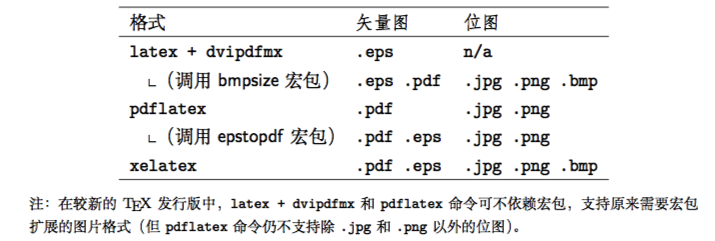
\includegraphics[width = 14cm]{Figure_13.png}
\caption{\LaTeX 各种编译方式支持的主流图片格式}
\end{figure}

在调用了 \ovalbox{graphicx} 宏包以后,就可以使用 \ovalbox{\textbackslash{}includegraphics} 命令加载图片了。












\end{document}